\chapter{Descripción teórica de técnicas de aprendizaje de métricas de distancia} \label{chapter:dml_algorithms}

En este capítulo se describen algunas de las técnicas más populares actualmente en el aprendizaje de métricas de distancia supervisado. A ellas se añade el análisis de componentes principales, pese a no ser supervisado, debido a su importancia para otros algoritmos de aprendizaje de métricas. Algunas estas técnicas, como PCA o LDA, constituyen procedimientos estadísticos desarrollados a finales del siglo pasado, que en la actualidad siguen siendo de gran relevancia en muchos problemas. Otras propuestas más recientes se sitúan en el estado del arte, como es el caso de NCMML o DMLMJ, entre otras.

Las técnicas analizadas se agrupan en seis secciones. Cada una de estas secciones describe algoritmos que comparten una misma finalidad principal, si bien las finalidades que describen cada sección no son exclusivas. En la primera sección se estudian las técnicas orientadas específicamente a la reducción de dimensionalidad. A continuación, se desarrollan las técnicas cuya finalidad es aprender distancias que mejoren el clasificador kNN, seguidas de aquellas que buscan mejorar los clasificadores basados en centroides. La cuarta sección incluye los métodos basados en la teoría de la información, especialmente en las divergencias, aprendiendo así distancias que acerquen o alejen determinadas distribuciones de probabilidad según la divergencia medida. Posteriormente se describen varios mecanismos de aprendizaje de distancias con objetivos menos específicos. Por último, se analizan las versiones basadas en kernels de algunos de los algoritmos anteriores, para trabajar en espacios de alta dimensionalidad.

Para cada una de las técnicas se analizará el problema que buscan resolver u optimizar, las formulaciones matemáticas de dichos problemas y los algoritmos propuestos para resolverlos.

\section{Técnicas de reducción de dimensionalidad}

\subsection{PCA}

El \emph{análisis de componentes principales} (PCA, \emph{Principal Component Analysis}) es una de las técnicas más populares de reducción de dimensionalidad en el ámbito del aprendizaje de métricas de distancia. Aunque se trata de una técnica de aprendizaje sin ningún tipo de supervisión, resulta necesario hablar de ella en este trabajo, por un lado por su gran relevancia, y más en particular, porque PCA es la herramienta de reducción de dimensionalidad por excelencia utilizada en los algoritmos de aprendizaje de distancias supervisados que no admiten de por sí una reducción de dimensionalidad. En tales algoritmos, PCA se aplica primeramente sobre los datos para poder utilizar posteriormente el algoritmo en el espacio de dimensión reducida.

El análisis de componentes principales puede entenderse desde dos puntos de vista diferentes, que acaban conduciendo al mismo problema de optimización. El primero de estos enfoques consiste en encontrar dos transformaciones, una que comprima los datos a un espacio de menor dimensión, y otra que los descomprima en el espacio original, de forma que en el proceso de compresión y descompresión se pierda la mínima información.

Vamos a centrarnos en este primer enfoque. Supongamos que tenemos el conjunto de datos $\mathcal{X} = \{x_1,\dots,x_N\} \subset \mathbb{R}^d$, y fijamos $d' < d$. Vamos a suponer además que los datos están centrados, es decir, que su media es cero. Si no lo fuera, basta con aplicar previamente a los datos la transformación $x \mapsto x - \mu$, donde $\mu = \sum x_i / N$ es la media de los datos. Buscamos una matriz de compresión $L \in \mathcal{M}_{d'\times d}(\R)$ y una matriz de descompresión $U \in \mathcal{M}_{d\times d'}(\R)$ de forma que, tras comprimir y descomprimir cada dato, los cuadrados de las distancias euclídeas al dato original sean mínimos. Es decir, el problema que buscamos resolver es

\begin{equation} \label{eq:pca:compress}
    \min_{\substack{L \in \mathcal{M}_{d'\times d}(\R) \\ U \in \mathcal{M}_{d\times d'}(\R)}} \quad \sum_{i=1}^{N} \|x_i - ULx_i\|_2^2.
\end{equation}

Para encontrar una solución a este problema, en primer lugar vamos a ver que las matrices $U$ y $L$ han de estar relacionadas de una forma muy particular.

\begin{lem}
    %% **** Tal vez seria mejor poner existe una solucion (U,L) del problema tal que ...
    Si $(U,L)$ es una solución del problema \ref{eq:pca:compress}, entonces $LL^T = I$ (en $\mathbb{R}^{d'}$) y $U = L^T$.
\end{lem}

\begin{proof}
    Fijamos $U \in \mathcal{M}_{d\times d'}(\R)$ y $L \in \mathcal{M}_{d'\times d}(\R)$. Podemos suponer que tanto $U$ como $L$ tienen rango máximo, pues en caso contrario el rango de $UL$ es menor que $d'$. Notemos que en tal caso, siempre es posible extender las matrices $U$ y $L$ a rango máximo de forma que el subespacio generado extienda al generado por $UL$ (basta sustituir los vectores linealmente dependientes en las columnas de la matriz por vectores independientes mientras la dimensión lo permita), y en tal caso el error obtenido en \ref{eq:pca:compress} para la extensión va a ser, a lo sumo, el error obtenido para $U$ y $L$.

    Consideramos la aplicación $x \mapsto ULx$. La imagen de esta aplicación, $R = \{ ULx \colon x \in \R^d \}$, es un subespacio vectorial de $\R^d$ de dimensión $d'$. Sea $\{u_1,\dots,u_{d'}\}$ una base ortonormal de $R$, y sea $V \in \mathcal{M}_{d'\times d}(\R)$ la matriz que tiene, por filas, los vectores $u_1,\dots,u_{d'}$. Se verifica entonces que la imagen de $V$ tiene rango $d'$ y que $VV^T = I$. Además, si consideramos $V^T$ como aplicación lineal, se tiene que su imagen es $R$ (puesto que $V^Te_i = u_i, i = 1,\dots,d'$, donde $\{e_1,\dots,e_{d'}\}$ es la base usual de $\mathbb{R}^{d'}$).

    Por tanto, todos los vectores de $R$ pueden escribirse como $V^Ty$, con $y \in \mathbb{R}^{d'}$. Dados $x \in \R^d, y \in \R^{d'}$, se tiene
    \begin{align*}
    \|x-V^Ty\|_2^2 &= \langle x- V^Ty, x - V^Ty \rangle \\
                   &= \|x\|^2 - 2\langle x,V^T y\rangle + \|V^Ty\|^2 \\
                   &= \|x\|^2 - 2\langle y,Vx \rangle + y^TVV^Ty \\
                   &= \|x\|^2 - 2\langle y,Vx \rangle + y^Ty \\
                   &= \|x\|^2 + \|y\|^2 - 2 \langle y,Vx \rangle.
    \end{align*}

    Si calculamos el gradiente respecto de $y$ a partir de la última expresión anterior, obtenemos $\nabla_y \|x-V^Ty\|_2^2 = 2y - 2Vx$, que, al igualar a cero, nos permite obtener un único punto crítico, $y = Vx$. La convexidad de esta función (es la composición de la norma euclídea con una aplicación afín) nos asegura que este punto crítico es un mínimo global. Por tanto, esto nos indica que, para cada $x \in \R^d$, la distancia a $x$ en el conjunto $R$ alcanza su mínimo en el punto $V^TVx$. En particular, para los datos del conjunto $\mathcal{X}$ concluimos que
    \[ \sum_{i=1}^N \|x_i - ULx_i\|_2^2 \ge \sum_{i=1}^N\|x_i - V^TV x_i\|^2_2. \]

    Podemos encontrar una matriz $V$ con estas propiedades para cualesquiera $U$ y $L$ en las condiciones del problema, lo que concluye la prueba.
\end{proof}

El lema anterior nos permite reformular nuestro problema en términos únicamente de la matriz $L$,

\begin{equation} \label{eq:pca:compress2}
    \min_{\substack{L \in \mathcal{M}_{d'\times d}(\R) \\LL^T = I}} \quad \sum_{i=1}^{N} \|x_i - L^TLx_i\|_2^2.
\end{equation}

Notemos ahora que, para $x \in \R^d$ y $L \in \mathcal{M}_{d'\times d}(\R)$ con $LL^T = I$, se verifica
\begin{align*}
    \|x - L^TLx\|_2^2 &= \langle x - L^TLx, x - L^TLx \rangle \\
                      &= \|x\|^2 - 2\langle x,L^TLx \rangle + \langle L^TLx, L^TLx \rangle \\
                      &= \|x\|^2 - 2x^TL^TLx + x^TL^TLL^TLx \\
                      &= \|x\|^2 - x^TL^TLx \\
                      &= \|x\|^2 - \tr(x^TL^TLx) \\
                      &= \|x\|^2 - \tr(Lxx^TL^T).
\end{align*}

Por tanto, si eliminamos los términos que no dependen de $L$, podemos transformar el problema \ref{eq:pca:compress2} en el siguiente problema equivalente:
\begin{equation} \label{eq:pca:traceproblem}
    \max_{\substack{L \in \mathcal{M}_{d'\times d}(\R) \\LL^T = I}} \quad \tr\left(L \Sigma L^T\right),
\end{equation}

donde $\Sigma = \sum_{i=1}^N x_ix_i^T$ es, salvo una constante, la matriz de covarianza asociada a los datos de $\mathcal{X}$. Esta matriz es simétrica, y el teorema \ref{thm:eigen_trace_opt} garantiza que podemos encontrar un máximo del problema si construimos $L$ añadiendo los $d'$ vectores propios de $\Sigma$ correspondientes a sus $d'$ mayores valores propios. Estos vectores los podemos tomar ortonormales, por la simetría de $\Sigma$. Las direcciones que determinan estos vectores son las \emph{direcciones principales}, y las componentes de los datos transformados en el sistema ortonormal determinado por las direcciones principales son las llamadas \emph{componentes principales}.

Para concluir, el segundo enfoque desde el que se puede tratar el problema de los componentes principales consiste en la selección de las direcciones ortogonales para las que se maximice la varianza. Sabemos que si $\Sigma$ es la matriz de covarianza de $\mathcal{X}$, al aplicar una transformación $L$ a los datos la nueva matriz de covarianza viene dada por $L\Sigma L^T$. Si queremos una transformación que reduzca la dimensionalidad y para la cual se maximice la varianza en cada variable lo que buscamos es tomar la traza de la matriz anterior, lo que nos conduce de nuevo al problema \ref{eq:pca:traceproblem}. La simetría de $\Sigma$ garantiza que podamos tomar las direcciones principales ortonormales que maximicen la varianza para cada posible valor de $d'$.

Por último, es importante destacar que la matriz $L \in \mathcal{M}_{d}(\R)$ (tomando todas las dimensiones) que se construye añadiendo por filas los vectores propios de $\Sigma$ es la matriz ortonormal que diagonaliza $\Sigma$, y por tanto, al aplicar $L$ sobre los datos, los datos transformados tienen como matriz de covarianza la matriz diagonal $L\Sigma L^T = \diag(\lambda_1,\dots,\lambda_d)$, donde $\lambda_1,\dots,\lambda_d$ son los valores propios de $\Sigma$. Esto nos dice que los valores propios de la matriz de covarianza representan la cantidad de varianza explicada por cada una de las direcciones principales. Esto proporciona una ventaja adicional al PCA, ya que permite analizar el porcentaje de varianza que explica cada componente principal para poder a posteriori elegir una dimensión que se ajuste a la cantidad de varianza que se quiera conservar en los datos transformados.

La figura \ref{fig:pca} ejemplifica gráficamente el funcionamiento del análisis de componentes principales.

\begin{figure}[h]
    \centering
    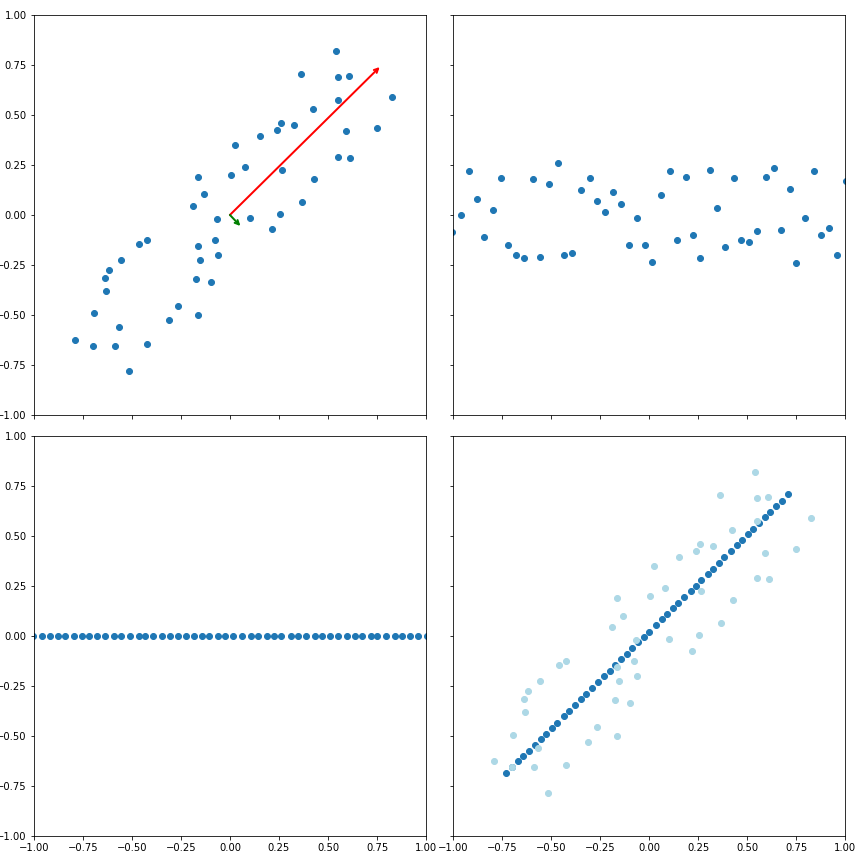
\includegraphics[width=0.75\textwidth]{./images/pca.png}
    \caption{Ejemplificación gráfica del PCA. En la primera imagen se muestra un conjunto de datos, junto con las direcciones principales (proporcionales de acuerdo a la varianza explicada) aprendidas por PCA. A su derecha, los datos proyectados en dimensión máxima. Observamos que dicha proyección consiste en girar los datos haciendo coincidir los ejes con las direcciones principales. Abajo a la izquierda, los datos proyectados sobre la primera componente principal. Por último, a su derecha, los datos recuperados mediante la matriz de descompresión, junto con los datos originales. Podemos comprobar que la proyección de PCA es la que minimiza el error cuadrático de descompresión. En este caso particular los datos descomprimidos se encuentran en la recta de regresión de los datos originales, debido a las dimensiones del problema.} \label{fig:pca}
\end{figure}

%% **** Figura(s) explicativa(s)

\subsection{LDA}

El análisis discriminante lineal (LDA, \emph{Linear Discriminant Analysis}) es una técnica clásica de aprendizaje de métricas de distancia cuya finalidad es aprender una matriz de proyección que maximice la separación entre clases en el espacio proyectado, es decir, trata de encontrar las direcciones que mejor permiten distinguir las distintas clases, como se muestra en la figura \ref{fig:lda}.

\begin{figure}[h]
    \centering
    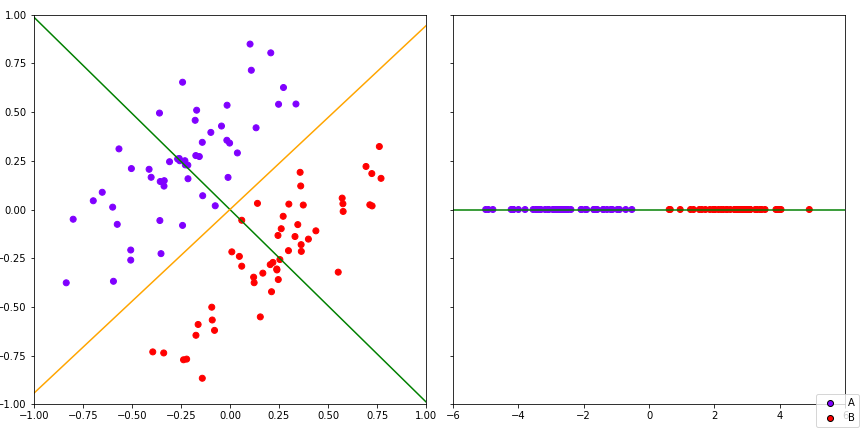
\includegraphics[width=0.75\textwidth]{./images/lda.png}
    \caption{Ejemplo gráfico del LDA y comparación con PCA. En la primera imagen se muestra un conjunto de datos, con la dirección principal determinada por PCA, en naranja, y la dirección determinada por LDA, en verde. Observamos que si proyectamos los datos sobre la dirección obtenida por LDA quedan bien separados, como se muestra en la imagen derecha. En cambio, la dirección obtenida por PCA solo nos permite maximizar la varianza de todo el conjunto al proyectar, pues no considera la información de las etiquetas.} \label{fig:lda}
    %
\end{figure}


La figura \ref{fig:lda} nos permite, además, comparar los resultados de las proyecciones obtenidas por PCA y LDA, mostrando la diferencia más notable entre ambas técnicas: PCA no tiene en cuenta la información de las clases, buscando las direcciones que maximizan la varianza del conjunto total de datos, mientras que LDA sí que utiliza la información presente en las etiquetas, obteniendo direcciones en las que mejor se pueden proyectar los datos para tener una buena separación de clases. Se puede apreciar que las direcciones obtenidas por PCA y LDA no presentan ningún tipo de relación, siendo esta última la única de las dos que proporciona una proyección de los datos orientada al aprendizaje supervisado. 

También es posible observar en la figura \ref{fig:lda} que no tiene sentido buscar una segunda dirección independiente que siga maximizando la separación de las clases, mientras que en PCA siempre tiene sentido ir buscando inductivamente direcciones ortogonales que maximicen la varianza. Si el conjunto de datos mostrado en la figura tuviera una tercera clase, podríamos encontrar una segunda dirección que maximizara la separación entre clases, ofreciendo así la posibilidad de proyectar sobre el plano. En general, vamos a ver que si tenemos $r$ clases podremos encontrar como mucho (y siempre que lo permita la dimensión del espacio original) $r-1$ direcciones que maximicen la separación. Esto nos indica que las proyecciones que va a aprender LDA van a ser, en general, hacia una dimensión bastante baja, y siempre limitada por el número de clases en el conjunto de datos.

Supongamos el conjunto de datos etiquetados $\mathcal{X} = \{x_1,\dots,x_N\} \subset \R^d$ donde $\mathcal{C}$ es el conjunto de clases del problema, e $y_1,\dots,y_N \in \mathcal{C}$ son las etiquetas asociadas a cada dato de $\mathcal{X}$. Supongamos que el número de clases del problema es $|\mathcal{C}| = r$. Para cada $c \in \mathcal{C}$ definimos el conjunto $\mathcal{C}_c = \{ i \in \{1,\dots,N\} \colon y_i = c \}$, y $N_c = |\mathcal{C}_c|$. Consideramos los vectores media de cada clase,
\[\mu_c = \frac{1}{N_c} \sum_{i \in \mathcal{C}_c} x_i,\]
y el vector media de todo el conjunto de datos,
\[\mu = \frac{1}{N}\sum_{c \in \mathcal{C}}\sum_{i \in \mathcal{C}_c}x_i = \frac{1}{N}\sum_{i=1}^N x_i. \]

Vamos a definir dos matrices de dispersion, una entre clases (denominada \emph{between-class}), y otra entre los datos de mismas clases o intra-clase (denominada \emph{within-class}), notadas como $S_b$ y $S_w$, respectivamente. La matriz de dispersión entre clases se define como
\begin{equation}
    S_b = \sum_{c \in \mathcal{C}} N_c(\mu_c - \mu)(\mu_c - \mu)^T.
\end{equation}
Y la matriz de dispersión intra-clase,
\begin{equation}
    S_w = \sum_{c \in \mathcal{C}} \sum_{i \in \mathcal{C}_c}(x_i- \mu_c)(x_i - \mu_c)^T.
\end{equation}  

Notemos que estas matrices, representan, salvo constantes multiplicativas, las covarianzas entre los datos de las distintas clases tomando las medias como representantes de cada clase en el primer caso, y la suma, para cada clase, de las covarianzas para los datos de dicha clase, en el segundo caso. Como queremos maximizar la separación vamos a formular el problema de optimización como la búsqueda función de una proyección $L \in \mathcal{M}_{d'\times d}(\R)$ que maximice el cociente entre las varianzas entre clase y las varianzas intra clase determinadas por las matrices anteriores. El problema se establece como
\begin{equation} \label{eq:lda}
    \max_{\substack{L \in \mathcal{M}_{d'\times d}(\R) }} \quad \tr\left((LS_wL^T)^{-1}(L S_b L^T)\right).
\end{equation}


El teorema \ref{thm:eigen_trace_ratio_opt} nos asegura que para maximizar el problema \ref{eq:lda} $L$ ha de estar compuesta por los vectores propios asociados a los valores propios de mayor valor de $S_w^{-1}S_b$, siempre que $S_w$ sea invertible. En la práctica, esto ocurre en la mayoría problemas donde $N \gg d$, pues $S_w$ es la suma de $N$ productos tensoriales, cada uno de los cuales puede aportar una dimensión al rango. Si $N \gg d$ es probable que $S_w$ tenga rango máximo. Esto, junto a que $S_w$ es semidefinida positiva garantizarían que $S_w$ fuera definida positiva, entrando así en las hipótesis del teorema.

Es interesante destacar el parecido entre el problema de optimización \ref{eq:lda} y la expresión del índice de Calinski-Harabasz \cite{maulik2002performance}, un índice utilizado en clustering para medir la separación de las clases establecidas.

Por otra parte, notemos, como ya se adelantó al inicio de la sección, que a lo sumo podemos obtener $r-1$ vectores propios con valor propio asociado no nulo. Esto es debido a que $S_b$ tiene a lo sumo rango $r-1$, pues su rango coincide con el rango de la matriz $A$ que tiene por columnas los vectores $\mu_c - \mu$ (se verifica que $S_b = A \diag(N_{c_1},\dots,N_{c_r}) A^T$), lo que da como rango a lo sumo $r$, y dicha matriz presenta además la combinación lineal $\sum N_c(\mu_c- \mu) = 0$. Por tanto, $S_w^{-1}S_b$ también tiene a lo sumo rango $r-1$. En consecuencia, la matriz de proyección que maximiza el problema \ref{eq:lda} también va a tener, a lo sumo, este rango, luego la proyección va a quedar contenida en un espacio de dicha dimensión. Por tanto, la elección de una dimensión $d' > r-1$ no va a aportar ninguna información adicional a la que aporta la proyección en dimensión $r-1$.

Para concluir, aunque hemos visto que LDA permite reducir la dimensionalidad añadiendo información supervisada frente a la no supervisión de PCA, también puede presentar algunas limitaciones:

\begin{itemize}
 \item Si la muestra de datos es demasiado pequeña, la matriz de dispersión intra-clase puede ser singular, impidiendo el cálculo de $S_w^{-1}S_b$. En esta situación, se han propuesto diversos mecanismos para seguir adelante con esta técnica. Uno de los más utilizados consiste en regularizar el problema, considerando, en lugar de $S_w$, la matriz $S_w + \varepsilon I$, donde $\varepsilon > 0$, haciendo que $S_w + \varepsilon I$ sea definida positiva. El problema de la singularidad de $S_w$ también surge si hay atributos correlacionados. Este caso se puede evitar eliminando atributos redundantes en un preprocesado previo al aprendizaje.

 \item La definición de las matrices de dispersión asume en cierta medida que los datos en cada clase se distribuyen mediante gaussianas multivariante. Por tanto, si los datos presentaran otras distribuciones, la proyección aprendida podría no ser de calidad.

 \item Como ya se ha comentado, LDA solo permite la extracción de $r-1$ atributos, lo cual puede ser subóptimo en algunos casos, pues se podría perder bastante información.
\end{itemize}


\subsection{ANMM}

ANMM (\emph{Average Neighbor Margin Maximization}) \cite{anmm} es una técnica de aprendizaje de métricas de distancia orientada específicamente a la reducción de dimensionalidad. Sigue por tanto el mismo camino que los ya comentados PCA y LDA, intentando solventar algunas de las limitaciones que presentan estos últimos.

El objetivo de ANMM es aprender una transformación lineal $L \in \mathcal{M}_{d'\times d}(\mathbb{R})$, con $d' \le d$,  que proyecte los datos a un espacio de menor dimensión, de forma que se maximice la similitud entre elementos de la misma clase y la separación entre elementos de distintas clases, siguiendo el criterio de maximización de márgenes que vamos a mostrar a continuación.

Consideramos el conjunto de datos de entrenamiento $\mathcal{X} = \{x_1,\dots,x_N\} \subset \mathbb{R}^d$, con etiquetas $y_1,\dots,y_N$, y fijamos $\xi, \zeta \in \N$, y la distancia euclídea como distancia inicial. A partir de estas variables vamos a construir dos tipos de vecindarios.

\begin{definition}
    Sea $x_i \in \mathcal{X}$.
    
    Se define el \emph{$\xi$-vecindario homogéneo más cercano} de $x_i$ como el conjunto de los $\xi$ datos más cercanos a $x_i$ que están en su misma clase. Lo notaremos por $\mathcal{N}_i^o$.
    
    Se define el \emph{$\zeta$-vecindario heterogéneo más cercano} de $x_i$ como el conjunto de los $\zeta$ datos más cercanos a $x_i$ que están en clases distintas a la de $x_i$. Lo notaremos por $\mathcal{N}_i^e$.
\end{definition} 

Lo que va a tratar de maximizar ANMM es el concepto de margen promedio de vecindario, que definimos a continuación.

\begin{definition}
    Dado $x_i \in \mathcal{X}$, se define su margen promedio de vecindario, y se nota $\gamma_i$, como
    \begin{equation}
        \gamma_i = \sum\limits_{k \colon x_k \in \mathcal{N}_i^e} \frac{\|x_i - x_k \|^2}{|\mathcal{N}_i^e|} - \sum\limits_{j \colon x_j \in \mathcal{N}_i^o} \frac{\|x_i - x_j \|^2}{|\mathcal{N}_i^o|}.
    \end{equation}
    
    Se define el margen promedio (global) de vecindario como
    \begin{equation}
        \gamma = \sum_{i=1}^N \gamma_i.
    \end{equation}

    
\end{definition}

Observemos que, para cada $x_i \in \mathcal{X}$, su margen promedio representa la diferencia entre la distancia media de $x_i$ a sus vecinos heterogéneos y la distancia media de $x_i$ a sus vecinos homogéneos. Por tanto, la maximización de este margen permite, localmente, alejar los datos de distintas clases y atraer a aquellos de la misma clase. En la figura \ref{fig:average_neighbor_margin} se describe gráficamente el concepto de margen promedio de vecindario.

\begin{figure}[h]
    \centering
    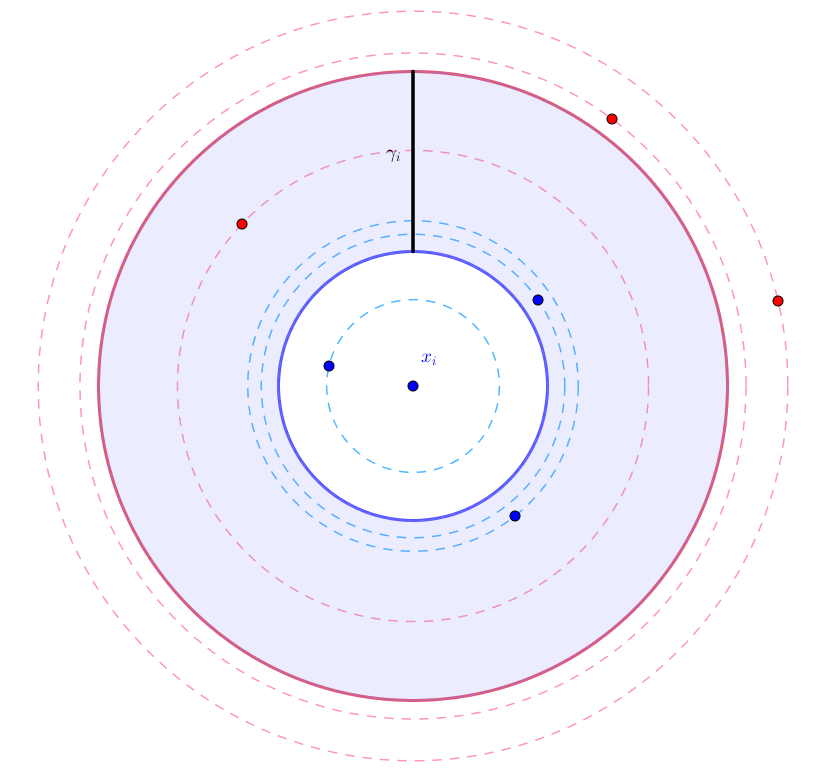
\includegraphics[width=0.55\textwidth]{./images/anmm.png}
    \caption{Descripción gráfica del margen promedio de vecindario para el dato $x_i$, para $\xi$ = $\zeta$ = 3. Las circunferencias azul y roja determinan la distancia media de $x_i$ a los datos de igual y distinta clase, respectivamente.} \label{fig:average_neighbor_margin}
\end{figure}

Buscamos ahora una transformación $L$ que maximice el margen asociado a los datos proyectados $\{Lx_i \colon i = 1,\dots,N\}$. Para tales datos, tenemos el margen asociado a dicha transformación,

\[ \gamma^L = \sum_{i=1}^{N} \gamma_i^L = \sum_{i=1}^N\left( \sum\limits_{k \colon x_k \in \mathcal{N}_i^e} \frac{\|Lx_i - Lx_k \|^2}{|\mathcal{N}_i^e|}- \sum\limits_{j \colon x_j \in \mathcal{N}_i^o} \frac{\|Lx_i - Lx_j \|^2}{|\mathcal{N}_i^o|} \right). \]

Notemos que, gracias a la linealidad de la traza, podemos expresar

\begin{align*}
    \sum_{i=1}^n\sum\limits_{k \colon x_k \in \mathcal{N}_i^e} \frac{\|Lx_i - Lx_k \|^2}{|\mathcal{N}_i^e|} &= \tr\left( \sum_{i=1}^N \sum\limits_{k \colon x_k \in \mathcal{N}_i^e} \frac{(Lx_i - Lx_k)(Lx_i - Lx_k)^T}{|N_i^e|} \right) \\
    &= \tr\left[ L \left( \sum_{i=1}^N \sum\limits_{k \colon x_k \in \mathcal{N}_i^e} \frac{(x_i-x_k)(x_i-x_k)^T}{|N_i^e|}  \right) L^T\right]\\
    &= \tr(LSL^T),
\end{align*}

donde $S = \sum_{i}\sum_{k\colon x_k \in \mathcal{N}_i^e}\frac{(x_i-x_k)(x_i-x_k)^T}{|\mathcal{N}_i^e|}$ recibe el nombre de matriz de dispersión. De la misma forma, si llamamos $C = \sum_{i}\sum_{j\colon x_j \in \mathcal{N}_i^o}\frac{(x_i-x_j)(x_i-x_j)^T}{|\mathcal{N}_i^o|}$, la cual denominaremos matriz de compacidad, se tiene que

\begin{equation*}
    \sum_{i=1}^n\sum\limits_{j \colon x_j \in \mathcal{N}_i^o} \frac{\|Lx_i - Lx_j \|^2}{|\mathcal{N}_i^o|} = \tr(LCL^T).
\end{equation*}

Y por tanto, combinando ambas expresiones,

\begin{equation} \label{eq:margin_caract}
    \gamma^L = \tr(L(S-C)L^T).
\end{equation}

La maximización de $\gamma^L$ tal como se presenta en la fórmula \ref{eq:margin_caract} no es lo suficientemente restrictiva, pues basta multiplicar $L$ por constantes positivas para obtener un valor de $\gamma^L$ tan grande como queremos. Por eso, se añade la restricción $LL^T = I$, por lo que acabamos obteniendo el siguiente problema de optimización:

\begin{align*}
    \max_{L \in \mathcal{M}_{d'\times d}(\R)} &\quad \tr\left(L(S-C)L^T\right)  \\
    \text{s.a.: } &\quad LL^T = I
\end{align*}

Notemos que $S - C$ es simétrica, pues es la diferencia de dos matrices semidefinidas positivas (cada una de ellas es suma de productos tensoriales). El teorema \ref{thm:eigen_trace_opt} nos dice que la matriz $L$ que buscamos la podemos construir añadiendo, por filas, los $d'$ vectores propios correspondientes a los $d'$ mayores valores propios de $S-C$.

Notemos que ANMM solventa alguna de las carencias de los ya vistos PCA y LDA. Por un lado, se trata de un algoritmo de aprendizaje supervisado, luego utiliza la información de las clases que es ignorada por PCA. Y frente a las carencias de LDA, podemos observar que:

\begin{itemize}
    \item No tiene problemas de cómputo con muestras pequeñas, para las cuales las matrices de dispersión o compacidad podrían resultar singulares, pues no tiene que calcular sus matrices inversas.
    \item No asume ninguna distribución sobre las clases.
    \item Admite cualquier tamaño para la reducción de dimensionalidad, no impone que dicho tamaño sea inferior al número de clases.
\end{itemize}

Por último, podemos observar también que, si mantenemos la dimensión máxima $d$, la condición $LL^T = I$ implica que $L$ es ortogonal y $L^TL=I$, luego estamos aprendiendo únicamente una isometría, como ya ocurría con PCA. Por ello, clasificadores basados en distancias como el kNN solo podrán experimentar mejoras cuando la dimensión escogida sea estrictamente menor que la original.


\section{Técnicas orientadas a la mejora del clasificador de vecinos cercanos}

\subsection{LMNN} \label{section:lmnn}

LMNN (\textit{Large Margin Nearest Neighbors}) \cite{lmnn} es un algoritmo de aprendizaje de métricas de distancia orientado específicamente a mejorar la precisión del clasificador kNN. Se basa en la premisa de que el kNN clasificará con más fiabilidad un ejemplo si sus $k$ vecinos comparten la misma etiqueta, y para ello intenta aprender una distancia que maximice el número de ejemplos que comparten etiqueta con el mayor número de vecinos posible.

De esta forma, el algoritmo LMNN trata de minimizar una función de error que penaliza, por un lado, las distancias grandes entre cada ejemplo y los considerados como sus vecinos ideales, y por otro lado, las distancias pequeñas entre ejemplos de distintas clases.

Supongamos que tenemos un conjunto de datos $\mathcal{X} = \{x_1,\dots,x_N\} \subset \mathbb{R}^d$ con etiquetas $y_1,\dots,y_N$. Para su funcionamiento, el algoritmo hace uso del concepto de \emph{vecinos objetivo} o \emph{target neighbors}. Dado un ejemplo $x_i \in \mathcal{X}$, sus $k$ vecinos objetivos son aquellos ejemplos de la misma clase que $x_i$, y distintos de este, para los que se desea que sean considerados como vecinos en la clasificación del kNN. Si $x_j$ es un vecino objetivo de $x_i$, entonces lo notaremos $j \istargetof i$. Estos vecinos objetivo están fijos durante el proceso de aprendizaje. Si se dispone de alguna información a priori se puede utilizar para determinarlos. En caso contrario, una buena opción es utilizar los vecinos cercanos de la misma clase para la distancia euclídea.

Una vez establecidos los vecinos objetivo, para cada distancia y para cada ejemplo que manejemos podemos establecer un perímetro determinado por el vecino más lejano a dicho ejemplo. Buscamos distancias para las cuales no haya ejemplos de otras clases en dicho perímetro. Hay que destacar que con este perímetro no hay suficientes garantías de separación, pues la distancia encontrada podría haber colapsado todos los vecinos objetivo en un punto y entonces el perímetro tendría radio cero. Por ello se considera un margen determinado por el radio del perímetro, al que se añade una constante positiva. Veremos que no hay pérdida de generalidad, por la función objetivo que vamos a definir, en suponer que dicha constante es 1. A cualquier ejemplo de distinta clase que invada este margen lo llamaremos \emph{impostor}. Nuestro objetivo, por tanto, será, además de acercar cada ejemplo a sus vecinos objetivo lo máximo posible, intentar alejar lo máximo posible a los impostores.

En términos matemáticos, si nuestra distancia está determinada por la aplicación lineal $L \in \mathcal{M}_{d}(\R)$, y $x_i, x_j \in \mathcal{X}$ con $j \istargetof i$, diremos que $x_l \in \mathcal{X}$ es un impostor para los datos anteriores si $y_l \ne y_i$ y $\|L(x_i - x_j)\|^2 \le \|L(x_i - x_j)\|^2+1$. En la figura \ref{fig:targets_impostors} se describen gráficamente los conceptos de vecino objetivo e impostor. Notemos por último que el margen está definido en términos de la distancia al cuadrado, en lugar de considerar solo la distancia. Esto facilitará la resolución del problema que vamos a formular.

\begin{figure}[h]
    \centering
    \begin{subfigure}{.5\textwidth}
        \centering
        \fbox{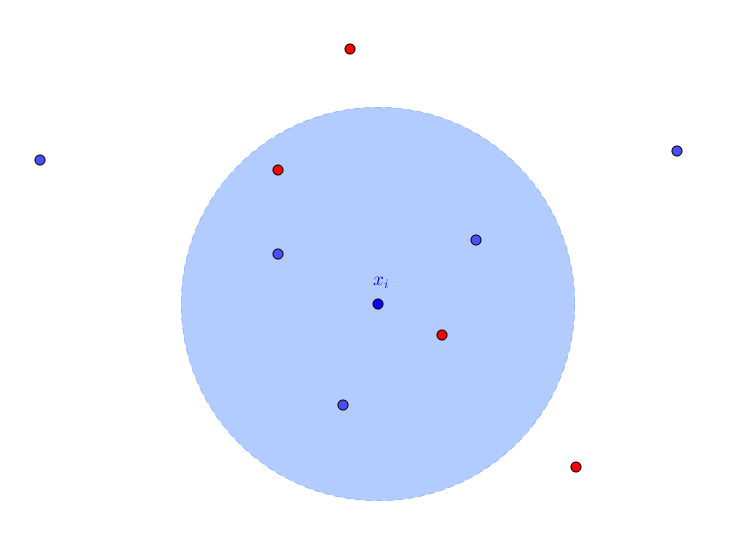
\includegraphics[height = 5cm]{images/lmnn1.png}}
    \end{subfigure}%
    \begin{subfigure}{.5\textwidth}
        \centering
        \fbox{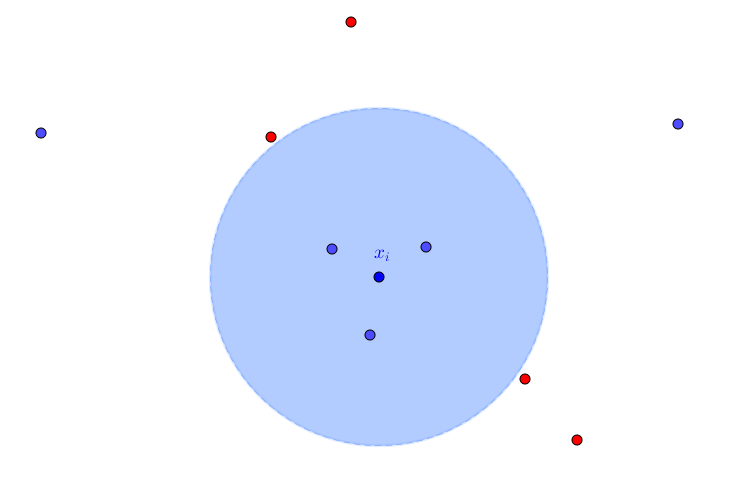
\includegraphics[height = 5cm]{images/lmnn2.png}}
    \end{subfigure}
    %\includegraphics[width=0.5\textwidth]{targets_impostors.png}
    \caption{Descripción gráfica de vecinos objetivo e impostores (para $k = 3$) para el dato $x_i$. El círculo azul representa el margen que determinan los vecinos objetivo. Todos los puntos de distintas clases en dicho círculo son impostores. El objetivo LMNN será acercar los vecinos objetivos lo máximo posible y eliminar los impostores del círculo. Por tanto, no influirán los datos de la misma clase que no sean vecinos objetivo y se dejarán de penalizar los impostores en cuanto salgan del margen, como se muestra a la derecha. Esto da un carácter local a esta técnica de aprendizaje.} \label{fig:targets_impostors}
\end{figure}

A continuación, procedemos a definir de forma precisa los términos de la función objetivo. Como ya se ha mencionado, va a estar compuesta de dos términos. El primero penalizará a los vecinos objetivo lejanos y el segundo penalizará a los impostores cercanos. El primer término se define como
\[ \varepsilon_{pull}(L) = \sum_{i=1}^N \sum_{j\istargetof i} \|L(x_i-x_j)\|^2. \]

Notemos que su minimización genera una fuerza de atracción entre los datos. El segundo término se define como
\[ \varepsilon_{push}(L) = \sum_{i=1}^{N}\sum_{j\istargetof i}\sum_{l=1}^{N} (1 - y_{il})[1 + \|L(x_i-x_j)\|^2 - \|L(x_i-x_l)\|^2]_{+}, \]

donde $y_{il}$ es una variable binaria, que vale $1$ y $y_i = y_l$ y $0$ si $y_i \ne y_l$, y el operador $[ \cdot ]_{+}\colon  \R \to \R^+_0$ se define como $[z]_{+} = \max\{z,0\}$. De esta forma, este error suma cuando $y_{il} = 0$ (es decir, $x_l$ es de distinta clase que $x_i$), y el segundo factor es estrictamente positivo (es decir, se sobrepasa el margen definido para los impostores). La minimización de este segundo término genera una fuerza de repulsión entre los datos.

Finalmente, la función objetivo resulta de combinar estos dos términos. Fijado $\mu \in ]0,1[$, definimos
\begin{equation} \label{eq:lmnn:L}
\varepsilon(L) = (1 - \mu)\varepsilon_{pull}(L) + \mu\varepsilon_{push}(L).
\end{equation}

Los autores afirman que, experimentalmente, la elección de $\mu$ no provoca grandes diferencias en los resultados, por lo que se suele tomar $\mu = 1/2$. La minimización de esta función nos llevará a aprender la distancia que buscábamos. Notemos que esta función no es convexa, por lo que si utilizamos un método de descenso bajo esta aproximación podemos quedar atrapados en un óptimo local. Sin embargo, podemos reformular nuestra función objetivo para que actúe sobre el cono de las matrices semidefinidas positivas. Si para cada $L \in \mathcal{M}_d(\R)$, tomamos $M = L^TL \in \mathcal{M}_d(\R)^+_0$, sabemos que $\|x_i-x_j\|_M^2 = \|x_i - x_j\|_L^2$, y por tanto,
\begin{equation} \label{eq:lmnn:M}
 \varepsilon(M) = (1-\mu) \sum_{i=1}^{N}\sum_{j\istargetof i} \|x_i - x_j\|_M^2 + \mu \sum_{i=1}^{N}\sum_{j\istargetof i}\sum_{l=1}^N [ 1 + \|x_i - x_j\|_M^2 - \|x_i - x_l\|_M^2]_{+}
\end{equation}

es una función convexa en $M$ que tiene toma los mismos valores que $\varepsilon(L)$. La minimización de $\varepsilon(M)$ en este caso está sujeta a la restricción $M \succeq 0$, por lo que podemos efectuarla mediante programación semidefinida, desplazándonos en la dirección del gradiente y proyectando el resultado sobre el cono semidefinido en sucesivas iteraciones. Además, podemos calcular un subgradiente $G \in \partial \varepsilon / \partial M$ dado por
\[ G = (1-\mu) \sum_{i,j\istargetof i} O_{ij} + \mu \sum_{(i,j,l) \in \mathcal{N}} (O_{ij} - O_{il}), \]

donde $\mathcal{N}$ es el conjunto de tripletas $(i,j,l)$ para las cuales $x_l$ es un impostor sobre $x_i$ con el margen determinado por $x_j$, y $O_{ij} = (x_i - x_j)(x_i - x_j)^T$ son los productos tensoriales obtenidos de derivar las distancias. El primer término del gradiente es constante, mientras que el segundo solo varía en cada iteración con los cambios de los impostores que entran o salen de el conjunto $\mathcal{N}$. Estas consideraciones permiten realizar un cálculo del gradiente bastante eficiente.

En cuanto a la reducción de dimensionalidad, se presentan dos alternativas diferentes. Si mantenemos la optimización respecto a $M$, no es factible añadir restricciones de rango y seguir obteniendo un problema de programación semidefinida. Por tanto, se propone el uso de PCA previamente a la ejecución del algoritmo, para proyectar los datos sobre sus componentes principales, y aplicar LMNN sobre los datos proyectados. La otra alternativa es optimizar la función objetivo respecto a $L \in \mathcal{M}_{d'\times d(\R)}$, con $d' < d$, usando algún algoritmo de gradiente descendente. En este caso la optimización no es convexa, pero aprendemos directamente una transformación lineal que reduce la dimensionalidad sin realizar cambios en el problema de optimización. Los autores afirman además, basados en los resultados empíricos, que esta optimización no convexa da buenos resultados.

Otras propuestas realizadas para la mejora de este algoritmo consisten en aplicar LMNN múltiples veces, aprendiendo así nuevas métricas cada vez, e ir utilizando estas métricas para determinar vecinos objetivo cada vez más precisos, o bien aprender métricas localmente. Por último, aunque la distancia aprendida está diseñada para que pueda ser utilizada por el kNN, también es posible utilizar la propia función objetivo como método para clasificar. Estos modelos de clasificación se denominan basados en energía. De este modo, para clasificar un dato test $x_t$, para cada posible valor de clase $y_t$, buscamos $k$ vecinos objetivo en el conjunto de entrenamiento de clase $y_t$, y evaluamos la \emph{energía} para la métrica aprendida, asignando finalmente a $x_t$ el valor de $y_t$ que proporcione menor energía. De acuerdo con la funión objetivo, la energía penalizará distancias grandes entre $x_t$ y sus vecinos objetivo, los impostores en el perímetro de $x_t$ y perímetros de otras clases invadidas por $x_t$. Por tanto,
\begin{equation}
\begin{split}
 y_t^{pred} &= \arg\min_{y_t} \left\{ (1-\mu) \sum_{j \istargetof t} \|x_t-x_j\|_M^2 \right. \\
            &+ \mu \sum_{j \istargetof t,l} (1-y_{tl})\left[ 1 + \|x_t-x_j\|_M^2 - \|x_t-x_l\|_M^2\right]_+  \\
            &+ \left. \mu \sum_{i,j \istargetof i}(1 - y_{it}) \left[ 1 + \|x_i-x_j\|_M^2 - \|x_i-x_t\|_M^2\right]_+ \right\} .
\end{split}
\end{equation}

\subsection{NCA}

\subsubsection{El kNN y la validación \emph{Leave One Out}}

En la mayoría de problemas de clasificación, para medir la eficacia del clasificador con el que estamos trabajando, se suele dividir el conjunto de datos del que disponemos en dos grupos: un conjunto de entrenamiento, que será el que utilice el clasificador para aprender, y un conjunto de validación, sobre el que el clasificador asigna sus predicciones, las cuales se comparan con las clases reales para evaluar el acierto del clasificador.

En algunos casos también puede resultar de interés evaluar el rendimiento del clasificador sobre los propios datos de entrenamiento, por ejemplo, para determinar si se está produciendo sobreaprendizaje, es decir, si el clasificador se adapta demasiado a los datos de entrenamiento, perdiendo así capacidad de generalización. Otra razón para ello es poder utilizar el rendimiento sobre los datos de entrenamiento como función objetivo a optimizar durante el proceso de aprendizaje. Esto contribuirá a mejorar el rendimiento del clasificador, siempre que no caiga en el sobreaprendizaje. Vamos a centrarnos en esta última razón.

En el caso del kNN, si pretendemos medir el rendimiento sobre los datos de entrenamiento, nos encontramos con un inconveniente que nos puede llevar a una interpretación incorrecta de los resultados. Y es que, para cada dato en el conjunto de entrenamiento, su vecino más cercano es él mismo, y por tanto, la clase que vaya a serle asignada va a estar condicionada por este hecho. Esto se aprecia más claramente en el caso $k=1$, donde el único vecino cercano considerado coincide siempre con el propio dato, y por tanto la tasa de acierto va a ser del 100 \%.

La forma de solucionar este inconveniente consiste en, si $\mathcal{X}$ es el conjunto de datos de entrenamiento, para cada $x \in \mathcal{X}$, obtener su predicción encontrando sus $k$ vecinos más cercanos en $X  \setminus \{x\}$. Esto es equivalente a particionar $X$ en conjuntos de un elemento, usando uno de los subconjuntos para la validación, y el resto para el entrenamiento. Este procedimiento de validación se conoce como validación cruzada \emph{Leave One Out} (LOO). Como procedimiento de validación en general, su estimación del error es poco sesgada y no tiene componente aleatoria, aunque está sometido a mayor variabilidad y es más costoso computacionalmente que otras técnicas de validación.

\subsubsection{El análisis de componentes de vecindarios}

NCA (\emph{Neighborhood Component Analysis}) \cite{nca} es un algoritmo de aprendizaje de métricas de distancia orientado específicamente a mejorar la precisión del clasificador kNN. Tiene como finalidad aprender una transformación lineal cuyo objetivo principal es minimizar el error \emph{Leave One Out} esperado por la clasificación mediante kNN. Adicionalmente, esta transformación podría usarse para reducir la dimensionalidad del conjunto de datos, y hacer por tanto más eficiente el clasificador.
    
Consideramos $\mathcal{X} = \{x_1,\dots,x_N\} \subset \mathbb{R}^d$ un conjunto de datos de entrenamiento con etiquetas $y_1,\dots,y_N$, respectivamente. Queremos aprender una distancia, determinada por una transformación lineal $L \in \mathcal{M}_{d}(\mathbb{R})$, que optimice la precisión del clasificador de vecinos cercanos. Lo ideal sería optimizar la actuación sobre los datos de validación, pero solo disponemos del conjunto de entrenamiento. Por tanto, nuestro objetivo va a ser optimizar el error \emph{Leave One Out} de clasificación sobre el conjunto de entrenamiento.

Sin embargo, la función que para cada $L$ asigna el error LOO para la distancia asociada a $L$ no tiene garantías de diferenciabilidad, ni siquiera de continuidad, por lo que no es fácil tratar con ella para su optimización (notemos que esta función toma un conjunto finito de valores y está definida en un conjunto conexo, luego no puede ser continua a menos que sea constante, lo cual no sucede en ejemplos no triviales).

Para ello, NCA trata de abordar el problema de forma estocástica, esto es, en vez de operar con el error LOO directamente, lo hace sobre su valor esperado para la probabilidad que vamos a definir a continuación.

Dados dos ejemplos $x_i, x_j \in \mathcal{X}$, definimos la probabilidad de que $x_i$ tenga a $x_j$ como su vecino más cercano para la distancia $L$ como
\begin{equation}
    \begin{split}
    p_{ij}^L = \frac{\exp\left( - \|Lx_i - Lx_j \|^2 \right)}{\sum\limits_{k \ne i} \exp\left(-\|Lx_i - Lx_k \|^2\right)}\ \ (j \ne i),  
    \end{split}
    \quad\quad
    \begin{split}
    p_{ii}^L = 0.
    \end{split}
\end{equation}

Notemos que, efectivamente, $p_{i*}$ define una medida de probabilidad sobre el conjunto $\{1,\dots,N\}$, para cada $i \in \{1,\dots,N\}$. Bajo esta ley de probabilidad, podemos definir la probabilidad de que el ejemplo $x_i$ esté correctamente clasificado como la suma de las probabilidades de que $x_i$ tenga como vecino más cercano a cada ejemplo de su misma clase, esto es,
\begin{equation}
    p_i^L = \sum_{j \in C_i} p_{ij}^L \text{, donde } C_i = \{j \in \{1,\dots,N\}\colon y_j = y_i\}.
\end{equation}

Finalmente, el número esperado de ejemplos correctamente clasificados, y la función que vamos a maximizar, la obtenemos como
\begin{equation}
    f(L) = \sum_{i=1}^N p_i^L = \sum_{i=1}^N \sum_{j \in C_i} p_{ij}^L = \sum_{i=1}^N \sum_{\substack{j \in C_i \\ j \ne i}} \frac{\exp\left(-\|Lx_i - Lx_j \|^2\right)}{\sum\limits_{k \ne i} \exp\left( -\|Lx_i - Lx_k\|^2 \right)}.
\end{equation}

Esta función sí es diferenciable, y su derivada es
\begin{equation}
    \frac{\partial f}{\partial L}(L) = 2L \sum_{i=1}^N \left( p_i^L \sum_{k=1}^N p_{ik}^L x_{ik}x_{ik}^T - \sum_{j \in C_i} p_{ij}^Lx_{ij}x_{ij}^T \right).
\end{equation}

Una vez obtenido el gradiente, podemos optimizar la función objetivo aplicando algún método de gradiente ascendente. Notemos que la función objetivo no es cóncava, y por tanto puede quedar atrapada en óptimos locales. Por otra parte, respecto al posible sobreajuste, los autores afirman que, basados en los resultados experimentales, no se produce sobreaprendizaje aunque se ascienda mucho en la función objetivo.

Finalmente, notemos que el mismo procedimiento es aplicable a cualquier matriz $L \in \mathcal{M}_{d'\times d}(\mathbb{R})$, con $d' < d$, por lo que NCA también puede ser utilizado para reducir la dimensionalidad de nuestro conjunto de datos.


\section{Técnicas orientadas a la mejora del clasificador de centroides cercanos}

\subsection{NCMML}

NCMML (\emph{Nearest Class Mean Metric Learning}) \cite{ncmml} es un algoritmo de aprendizaje de métricas de distancia orientado a mejorar específicamente el clasificador NCM. Para ello, utiliza un enfoque probabilístico simiar al utilizado por NCA para mejorar la precisión del kNN.

Consideramos el conjunto de datos de entrenamiento $\mathcal{X} = \{x_1,\dots,x_N\} \subset \R^d$, con etiquetas $y_1,\dots,y_N \in \mathcal{C}$, donde $\mathcal{C} = \{c_1,\dots,c_r\}$ es el conjunto de clases. Para cada $c \in \mathcal{C}$, llamamos $\mu_c \in \R^d$ al vector media de los datos pertenecientes a la clase $c$, es decir, $\mu_c = \frac{1}{N_c}\sum_{i\colon y_i = c}x_i$, donde $N_c$ es el número de elementos de $\mathcal{X}$ que pertenecen a la clase $c$. Dada una transformación lineal $L \in \mathcal{M}_{d'\times d}(\R)$, vamos a definir, para cada $x \in \mathcal{X}$ y cada $c \in \mathcal{C}$, la probabilidad de que $x$ sea etiquetado don la clase $c$ (de acuerdo con el criterio NCM) como
\begin{equation}
    p_L(c|x) = \frac{\exp\left(-\frac{1}{2} \|L(x - \mu_c)\|^2\right)}{\sum\limits_{c' \in \mathcal{C}} \exp\left(-\frac{1}{2} \|L(x - \mu_{c'})\|^2\right)}.
\end{equation} 

Notemos que efectivamente $p_L(\cdot|x)$ define una probabilidad en el conjunto $\mathcal{C}$. Una vez definida la probabilidad anterior, la función objetivo que trata de maximizar NCMML es el logaritmo de la verosimilitud para los datos etiquetados del conjunto de entrenamiento, esto es,
\begin{equation}
\mathcal{L}(L) = \frac{1}{N}\sum_{i=1}^N\log p_L(y_i|x_i).
\end{equation} 

Esta función es diferenciable y su gradiente viene dado por
\begin{equation}
\frac{\partial \mathcal{L}}{\partial L}(L) = \frac{1}{N} \sum_{i=1}^N \sum\limits_{c\in \mathcal{C}} \alpha_{ic} L (\mu_c - x_i)(\mu_c - x_i)^T,
\end{equation}

donde $\alpha_{ic} = p_L(c|x_i) - [\![ y_i = c ]\!]$ y $[\![ \cdot ]\!]$ denota la función indicadora de la condición $\cdot$. La maximización por métodos de gradiente de esta función es la tarea llevada a cabo por NCMML.



\subsection{NCMC} \label{section:ncmc}

\subsubsection{Generalizando NCM: El clasificador de múltiples centroides}

Aunque el clasificador NCM es un clasificador sencillo, intuitivo y eficiente tanto en el proceso de aprendizaje como el proceso de predicción, tiene un gran inconveniente, y es que presupone que las clases están agrupadas alrededor de su centro, lo cual es una hipótesis demasiado restrictiva. En la figura \ref{fig:problema_ncm} podemos ver un ejemplo en el que NCM es incapaz de dar buenos resultados.

\begin{figure}[h]
    \centering
    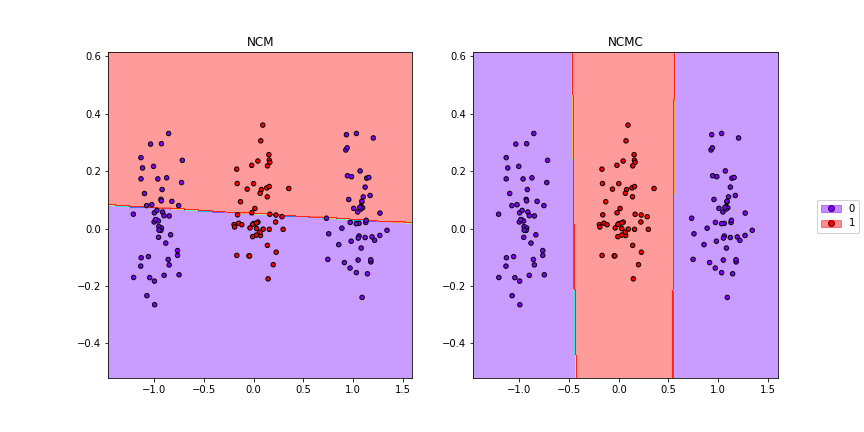
\includegraphics[width=1.0\textwidth]{images/ncm_problem.png}
    \caption{Conjunto de datos donde el clasificador NCM no da buenos resultados, pues los centroides de ambas clases son muy cercanos y ambos caen entre los puntos de la clase 1. Veremos que, escogiendo más de un centroide de forma adecuada podremos clasificar este conjunto como se muestra en la figura de la derecha.} \label{fig:problema_ncm}
\end{figure}

Una forma de solventar este problema es, en vez de considerar el centro de la clase para clasificar nuevos datos, encontrar subgrupos dentro de cada clase que presenten un agrupamiento de calidad, y para cada uno de estos subgrupos considerar su centro. Tendríamos de esta forma un conjunto de centroides para cada clase, y a la hora de clasificar un nuevo dato, bastaría seleccionar el centroide más cercano y asignarle la clase de la que es centroide.

Este nuevo clasificador, que denominaremos NCMC (\emph{Nearest Class Multiple Centroids}), entran en juego los algoritmos de segmentación o \emph{clustering}. Existen numerosos algoritmos \cite{clustering_algorithms} para obtener un conjunto de clusters dado un conjunto de datos, cada uno con sus ventajas e inconvenientes. Dada la forma de nuestro problema, en el que nos interesa además no solo obtener un conjunto de clusters para cada clase, sino además un centro para cada cluster, el algoritmo que reúne las condiciones más idóneas, además de ser sencillo y eficiente, es K-Means.

\subsubsection{K-Means y la búsqueda de centroides}

\emph{K-means} es uno de los algoritmos de \emph{clustering} más populares. La idea original de este algoritmo es, fijado un natural $k$, encontrar $k$ clusters, cada uno con un centroide, que minimicen una función de coste que depende de las distancias de los puntos del cluster a su centroide. Encontrar la solución a ese problema de optimización es un problema NP-hard, incluso para aproximarlo. En consecuencia, se utiliza comúnmente un algoritmo iterativo que garantiza la reducción de la función de coste en cada iteración, si bien los resultados que ofrece no son necesariamente los óptimos. Es por ello que normalmente se denomina K-means a este algoritmo iterativo, en lugar de a la minimización de la función objetivo asociada.

En primer lugar describimos la función objetivo. Consideramos el conjunto de datos $\mathcal{X} = \{x_1,\dots,x_N\} \subset \R^d$. La función objetivo dependerá de una familia de subconjuntos, $C_1,\dots,C_k$ que forman una partición de $\mathcal{X}$. A su vez, cada conjunto $C_i$ tendrá asociado un centroide $\mu_i$, que será aquel punto del espacio euclídeo $\mathbb{R}^d$ que minimice la suma de los cuadrados de las distancias de los elementos en $C_i$ a dicho centroide.  La función objetivo sumará los cuadrados de estas distancias para todos los clusters, quedando como se muestra a continuación:
\begin{equation} \label{eq:obj:kmeans}
    G(C_1,\dots,C_k) = \min_{\mu_1,\dots,\mu_k \in \R^d} \sum_{i=1}^{k}\sum_{x\in C_i} \|x-\mu_i\|^2.
\end{equation}

A continuación se describe el algoritmo iterativo que se utiliza normalmente para la búsqueda de los centroides. Inicialmente, se parte de unos centroides $\mu_1^{(0)},\dots,\mu_k^{(0)}$ escogidos al azar. En cada iteración $t$, se determina la partición $\{C_1^{(t)},\dots,C_k^{(t)}$ a partir de los centroides $\mu_1^{(t-1)},\dots,\mu_k^{(t-1)}$ de forma que a cada $x \in \mathcal{X}$ se le asigna el cluster del centroide más cercano. Finalmente, se calculan los nuevos centroides $\mu_1^{(t)},\dots,\mu_k^{(t)}$ como el vector media de los datos en $\{C_1^{(t)},\dots,C_k^{(t)}$, respectivamente. El proceso se repite hasta que en una iteración no se produzca ningún cambio en los clusters generados, momento en el que el algoritmo habrá convergido.

Como ya se ha mencionado, este algoritmo garantiza que la función objetivo \ref{eq:obj:kmeans} decrece conforme aumenta el número de iteraciones. A pesar de esto, no se puede asegurar que el algoritmo alcance un óptimo global (en ocasiones es posible incluso que ni siquiera se alcance un óptimo local). Sin embargo, el carácter aleatorio y la eficiencia del algoritmo permite realizar distintas ejecuciones eligiendo diferentes centroides iniciales, lo que facilita el encuentro de soluciones aceptables. 

Aunque se trata de un algoritmo eficiente y que en la práctica obtiene buenos resultados en la función objetivo, hay que destacar que es necesario especificar el número de clusters previamente. Los clusters que se obtienen con este algoritmo suelen tomar formas esféricas o similares, no siendo útiles para datos que presentan otros tipos de agrupaciones. También los datos más lejanos pueden condicionar en gran medida el valor de los centroides, y en consecuencia también el de los clusters.

Para la clasificación con NCMC, el uso de K-Means se reduce a aplicar el algoritmo de segmentación dentro de cada subconjunto de datos asociado a cada una de las clases del problema de clasificación. De esta forma obtenemos de forma sencilla el conjunto de centroides buscado para cada clase, y sobre el cual podemos realizar la clasificación de nuevos datos buscando simplemente el centroide más cercano. De nuevo se hace necesario establecer previamente el número de centroides para cada clase. Dichos números pueden estimarse realizando validación cruzada. 


\subsubsection{Aprendiendo distancias para NCMC}

Una vez definido el clasificador NCMC, el proceso de aprendizaje de distancias es análogo al de NCM. Siguiendo la notación utilizada en NCMML, en este caso, en lugar de un conjunto de centros de clase $\{\mu_c\}$, con $c \in \mathcal{C}$, disponemos de un conjunto de centroides, $\{m_{c_j}\}_{j=1}^{k_c}$, con $k_c \in \mathbb{N}$, para cada $c \in \mathcal{C}$. En este caso, las probabilidades asociadas a cada clase para la predicción correcta de $x \in \mathcal{X}$ vienen dadas por $p_L(c|x) = \sum_{j=1}^{k_c} p_L(m_{c_j}|x)$, donde son los centroides aquellos cuya probabilidad viene dada por la función softmax
\begin{equation}
    p_L(m_{c_j}|x) = \frac{\exp\left( -\frac{1}{2} \|L(x-m_{c_j})\|^2 \right)}{ \sum\limits_{c \in \mathcal{C}} \sum\limits_{i=1}^{k_c} \exp\left( -\frac{1}{2} \|L(x-m_{c_i})\|^2 \right) }.
\end{equation}

De nuevo, maximizamos el logaritmo de la verosimilitud, $\mathcal{L}(L) = \frac{1}{N}\sum_{i=1}^N p_L(y_i|x_i)$, cuyo gradiente en este caso viene dado por
\begin{equation*}
    \frac{\partial \mathcal{L}}{\partial L}(L) = \frac{1}{N} \sum_{i=1}^N \sum_{c \in \mathcal{C}} \sum_{j=1}^{k_c} \alpha_{ic_j} L (m_{c_j}-x_i)(m_{c_j}-x_i)^T,
\end{equation*}
donde $\alpha_{ic_j} = p_L(m_{c_j}|x_i) - [\![ y_i = c ]\!] \frac{p_L(m_{c_j}|x_i)}{\sum_{j'=1}^{k_c} p_L(m_{c_{j'}}|x_i)}$. La maximización de la verosimilitud por métodos de gradiente es la tarea llevada a cabo por la técnica de aprendizaje de distancias para NCMC, que denominaremos con el mismo nombre que dicho clasificador.





\section{Técnicas basadas en teoría de la información}

\subsection{ITML}

ITML (\emph{Information Theoretic Metric Learning}) \cite{itml} es una técnica de aprendizaje de métricas de distancia cuyo objetivo es encontrar una métrica lo más cercana posible a una distancia de partida, entendiendo la cercanía desde el punto de vista de la entropía relativa, como formularemos más adelante, haciendo que dicha métrica satisfaga determinadas restricciones de similitud para los datos entrenados.

ITML parte de un conjunto de datos $\mathcal{X} = \{x_1,\dots,x_N\} \subset \R^d$, no necesariamente etiquetados, pero del que se conoce que determinados pares de datos considerados similares deben estar a una distancia menor o igual que $u$, y otros pares de datos considerados no similares deben estar situados a una distancia mayor o igual que $l$, donde $u$ y $l$ son constantes prefijadas de antemano, con valores relativamente pequeño y grande, respectivamente, respecto al conjunto de datos.

A partir de los datos con las restricciones indicadas, ITML considera una métrica inicial asociada a una matriz $M_0$ definida positiva, y trata de encontrar una matriz definida positiva $M$, lo más parecida posible a $M_0$, y que respete las restricciones de similitud impuestas. La forma de medir el parecido entre $M$ y $M_0$ se realiza utilizando herramientas de la teoría de la información.

Es conocido que hay una correspondencia entre las matrices definidas positivas y las distribuciones normales multivariante, fijado un mismo vector media $\mu$. Dada $M \in \mathcal{M}_d(\R)^+$, podemos construir una distribución normal a través de su función de densidad,
\[ p(x;M) = \frac{1}{(2\pi)^{n/2}\det(M)^{1/2}}\exp\left( (x-\mu)^TM^{-1}(x-\mu) \right). \]
Recíprocamente, a partir de dicha distribución, si calculamos la matriz de covarianza recuperamos la matriz $M$. Usando esta correspondencia, vamos a medir la cercanía entre $M_0$ y $M$ a través de la divergencia KL entre sus correspondientes gaussianas,
\[ \kl(p(x;M_0))\|p(x;M)) = \int p(x;M_0)\log\frac{p(x;M_0)}{p(x;M)}dx. \]

Una vez definido el mecanismo con el que vamos a medir la cercanía de las métricas, podemos establecer la formulación del problema a optimizar por la técnica ITML. Si denominamos $S$ y $D$ a los conjuntos de pares de índices sobre los elementos de $\mathcal{X}$ que representan a los datos considerados similares y no similares, respectivamente, y partimos de la métrica inicial $M_0$, el problema es
\begin{equation} \label{eq:itml:prob1}
    \begin{split}
    \min_{M \succeq 0} &\quad \kl(p(x;M_0)\|p(x;M))  \\
    \text{s.a.: } &\quad d_M(x_i,x_j) \le u, \quad (i,j) \in S \\
                  &\quad d_M(x_i,x_j) \ge l, \quad (i,j) \in D.
    \end{split}
\end{equation}

Para tratar este problema computacionalmente, se hace uso de la divergencia matricial \emph{log-det}, la cual viene dada por
\[ D_{ld}(M\|M_0) = \tr(MM_0^{-1}) - \log\det(MM_0^{-1}) -d, \quad M,M_0 \in \mathcal{M}_d(\R)^+. \]

Hemos visto en el teorema \ref{prop:caract_kl:2} que la divergencia KL entre dos gaussianas con la misma media se puede expresar en términos de la divergencia \emph{log-det} como
\[ \kl(p(x;M_0)\|p(x;M)) = \frac{1}{2}D_{ld}(M_0\|M). \]

Esto nos permite reformular el problema \ref{eq:itml:prob1} de la siguiente forma:
\begin{equation} \label{eq:itml:prob2}
    \begin{split}
    \min_{M \succeq 0} &\quad D_{ld}(M_0\|M)  \\
    \text{s.a.: } &\quad \tr(M(x_i-x_j)(x_i-x_j)^T) \le u, \quad (i,j) \in S \\
                  &\quad \tr(M(x_i-x_j)(x_i-x_j)^T) \ge l, \quad (i,j) \in D.
    \end{split}
\end{equation}

Es posible que no se pueda encontrar una métrica que satisfaga simultáneamente todas las restricciones, por lo que el problema podría no tener solución. Por ello, ITML introduce en el problema \ref{eq:itml:prob2} variables de holgura mediante las cuales se obtiene un problema en cuya optimización se establece un equilibrio entre la minimización de la divergencia y la satisfacción de las restricciones, para poder llegar así a una solución aproximada del problema original, en caso de no tener solución. Finalmente, la técnica computacional utilizada en la resolución de este problema de optimización es la conocida como el método de las \emph{proyecciones de Bregman} \cite{bregman_projections}, el cual es una generalización del método de las proyecciones iteradas.
%% *** Completar cuando se haga el tema de teoría de la información.

\subsection{DMLMJ}

DMLMJ (\emph{Distance Metric Learning through the maximization of the Jeffrey divergence}) \cite{dmlmj} es una técnica de aprendizaje de métricas de distancia basada, al igual que ITML, en conceptos de teoría de la información. Concretamente, la herramienta que utiliza es la conocida como divergencia de Jeffrey, a través de la cual pretende separar lo máximo posible la distribución asociada a los puntos similares de aquella asociada a los puntos no similares, en los términos que veremos a continuación.

Consideramos el conjunto de entrenamiento $\mathcal{X} = \{x_1,\dots,x_N\} \subset \R^d$ con correspondientes etiquetas $y_1,\dots,y_N$, y fijamos $k \in \N, k \ge 1$. Como ya hemos comentado, DMLMJ busca maximizar, respecto a la divergencia de Jeffrey, la separación entre las distribuciones de puntos similares y no similares. Para ello, introduciremos los siguientes conceptos:

\begin{definition}
    Dado $x_i \in \mathcal{X}$, el \emph{vecindario $k$-positivo} de $x_i$ se define como el conjunto de los $k$ vecinos más cercanos de $x_i$ en $\mathcal{X} \setminus \{x_i\}$ cuya clase es la misma que la de $x_i$. Se nota por $V_k^+(x_i)$.

    El \emph{vecindario $k$-negativo} de $x_i$ se define como el conjunto de los $k$ vecinos más cercanos de $x_i$ en $\mathcal{X}$ cuya clase es distinta de la de $x_i$. Se nota por $V_k^-(x_i)$.

    Se define el \emph{espacio de diferencias $k$-positivo} del conjunto de datos etiquetados como el conjunto 
    \[ S = \{x_i - x_j \colon x_i \in \mathcal{X}, x_j \in V_k^+(x_i)\}. \]

    Análogamente, se define el \emph{espacio de diferencias $k$-negativo} como el conjunto
    \[ D = \{x_i - x_j \colon x_i \in \mathcal{X}, x_j \in V_k^-(x_i)\}. \]

\end{definition}

Los conjuntos $S$ y $D$ representan, por tanto, los vectores con las diferencias entre los datos y sus $k$ vecinos más cercanos, de igual o de distinta clase, respectivamente. Llamamos $P$ y $Q$ a las distribuciones en los espacios $S$ y $D$, respectivamente, asumiendo que son gaussianas multivariante. Asumiremos, además, que ambas distribuciones tienen media 0. Esta asunción es razonable, puesto que en la práctica, en la mayoría de los casos, si $x_i$ es vecino de $x_j$, $x_j$ también lo es de $x_i$, luego ambas diferencias aparecerán en el espacio de diferencias, haciendo la media cero. Por último, llamaremos a las correspondientes matrices de covarianza $\Sigma_S$ y $\Sigma_D$, respectivamente.

Si ahora aplicamos una transformación lineal a los datos, $x \mapsto Lx$, con $L \in \mathcal{M}_{d'\times d}(\R)$, las distribuciones transformadas seguirán teniendo media 0 y covarianzas $L\Sigma_S L^T$ y $L\Sigma_D L^T$, respectivamente. A dichas distribuciones las denominaremos $P_L$ y $Q_L$. El objetivo de DMLMJ es encontrar una transformación que maximice la divergencia de Jeffrey entre $P_L$ y $Q_L$:
\[ \max_{L \in \mathcal{M}_{d'\times d}(\R)} \quad f(L) =  \jf(P_L\|Q_L) = \kl(P_L\|Q_L) + \kl(Q_L\|P_L).\]

Como se demostró en la proposición \ref{prop:caract_jeffrey:2}, la divergencia de Jeffrey entre las distribuciones gaussianas $P_L$ y $Q_L$ se puede expresar como 
\[ f(L) = \frac{1}{2} \tr\left( (L\Sigma_S L^T)^{-1} (L\Sigma_D L^T) + (L \Sigma_D L^T)^{-1} (L \Sigma_S L^T) \right) - d'. \]

Como $d'$ es constante, obtenemos el problema equivalente
\[ \max_{L \in \mathcal{M}_{d'\times d}(\R)} \quad J(L) =  \tr\left( (L\Sigma_S L^T)^{-1} (L\Sigma_D L^T) + (L \Sigma_D L^T)^{-1} (L \Sigma_S L^T) \right).\]

Si calculamos el gradiente de la función anterior, obtenemos
\[ \nabla J(L) = \left( 2 \Sigma_D L^T\Sigma_{2S}^{-1} - 2\Sigma_S L^T \Sigma_{2S}^{-1}\Sigma_{2D}\Sigma_{2S}^{-1} \right) + \left( 2\Sigma_S L^T \Sigma_{2D}^{-1} - 2 \Sigma_D L^T \Sigma_{2D}^{-1}\Sigma_{2S} \Sigma_{2D}^{-1} \right),\]
donde $\Sigma_{2S} = L \Sigma_S L^T$ y $\Sigma_{2D} = L\Sigma_D L^T$.

Cada uno de los términos entre paréntesis se anula, respectivamente, cuando $\Sigma_S^{-1} \Sigma_D L^T = L^T \Sigma_{2S}^{-1} \Sigma_{2D}$ y cuando $\Sigma_{D}^{-1}\Sigma_S L^T = L^T \Sigma_{2D}^{-1} \Sigma_{2S}$. Queremos resolver estas dos ecuaciones. Para ello, enunciamos los siguientes resultados.

\begin{thm}

    Sean $\Sigma_1, \Sigma_2 \in \mathcal{M}_d(\R)^+$ y sea $L \in \mathcal{M}_{d'\times d}(\R)$ una matriz que contiene, por filas, $d'$ vectores propios linealmente independientes de $\Sigma_1^{-1}\Sigma_2$. Entonces,
    \begin{equation} \label{eq:jef:thm1}
        \Sigma_1^{-1}\Sigma_2L^T = L^T(L\Sigma_1L^T)^{-1}(L\Sigma_2L^T).
    \end{equation}
\end{thm}

\begin{proof} \label{thm:dmlmj1}
    Sea $D \in \mathcal{M}_{d'}(\R)$ la matriz diagonal que contiene, en el mismo orden, los $d'$ valores propios de $\Sigma_1^{-1}\Sigma_2$ asociados a los vectores propios presentes en $L$. Se verifica entonces
    \begin{equation}\label{eq:jef:formula_vp}
        \Sigma_1^{-1}\Sigma_2L^T = L^TD.
    \end{equation} 

    Si multplicamos a ambos lados por $L\Sigma_1$, obtenemos
    \[ L\Sigma_2L^T = L\Sigma_1L^TD. \]

    $L\Sigma_1L^T$ es una matriz regular. Puesto que $\Sigma_1$ es definida positiva, admite una descomposición $\Sigma_1 = PP^T$, con $P$ regular de dimensión $d$. Entonces, $L\Sigma_1L^T = LPP^TL^T = LP(LP)^T$, donde $LP$ es una matriz cuadrada de dimensión $d'$ y de rango $d'$, por ser la composición (viéndolas como aplicaciones lineales) de un isomorfismo con una aplicación de rango $d'$, haciendo que la imagen tenga de nuevo dimensión $d'$. En consecuencia, $LP$ es regular, y por tanto también lo es $LP(LP)^T = L\Sigma_1L^T$, por lo que podemos tomar inversas, obteniendo
    \begin{equation} \label{eq:jef:coro1_pre}
        (L\Sigma_1L^T)^{-1}(L\Sigma_2L^T) = D.
    \end{equation}

    Si a continuación multiplicamos a la izquierda por $L^T$ en ambos lados de la igualdad, se tiene
    \[ L^T(L\Sigma_1L^T)^{-1}(L\Sigma_2L^T) = L^TD. \]

    Sustituyendo lo que acabamos de obtener en el lado derecho de \ref{eq:jef:formula_vp}, concluimos que
    \[\Sigma_1^{-1}\Sigma_2L^T = L^T(L\Sigma_1L^T)^{-1}(L\Sigma_2L^T).\]

\end{proof}

\begin{cor} \label{cor:dmlmj1}
    Sean $\Sigma_1, \Sigma_2 \in \mathcal{M}_d(\R)^+$ y sea $L \in \mathcal{M}_{d'\times d}(\R)$ una matriz que contiene, por filas, $d'$ vectores propios linealmente independientes de $\Sigma_1^{-1}\Sigma_2$. Sea $D \in \mathcal{M}_{d'}(\R)$ la matriz diagonal con los correspondientes $d'$ valores propios. Entonces,
    \[ \tr\left( (L\Sigma_1L^T)^{-1}(L\Sigma_2L^T) \right) = \tr(D). \]
\end{cor}

\begin{proof}
    Basta tomar trazas en la igualdad de matrices de la ecuación \ref{eq:jef:coro1_pre}.
    \begin{comment}
    Se verifica de nuevo la ecuación \ref{eq:jef:formula_vp}. Combinándola con la ecuación \ref{eq:jef:thm1} del teorema anterior, se tiene
    \[ L^T(L\Sigma_1L^T)^{-1}(L\Sigma_2L^T) = L^TD. \]

    $L^T$ es una matriz de dimensión $d\times d'$, con $d' \le d$ y de rango máximo, luego admite una inversa por la izquierda. Multiplicando por dicha inversa, obtenemos
    \[ (L\Sigma_1L^T)^{-1}(L\Sigma_2L^T) = D.\]

    La prueba concluye al tomar trazas en esta última igualdad de matrices.
    \end{comment}
\end{proof}

De acuerdo con el teorema \ref{thm:dmlmj1}, podemos observar que es posible anular simultáneamente ambos términos del gradiente tomando $L$ como una matriz de vectores propios de $\Sigma_S^{-1}\Sigma_D$, o bien de $\Sigma_D^{-1}\Sigma_S$. Notemos que ambos casos comparten los mismos vectores propios y cada opción tiene como valores propios los inversos de la opción restante. Optamos por tomar $d'$ vectores propios del primer caso, de $\Sigma_S^{-1}\Sigma_D$. Entonces, $\nabla J(L) = 0$ y el corolario \ref{cor:dmlmj1} nos dice que
\begin{align*}
    J(L) &= \tr\left( (L\Sigma_S L^T)^{-1} (L\Sigma_D L^T) + (L \Sigma_D L^T)^{-1} (L \Sigma_S L^T) \right) \\
         &= \tr\left( (L\Sigma_S L^T)^{-1} (L\Sigma_D L^T)\right) + \tr\left((L \Sigma_D L^T)^{-1} (L \Sigma_S L^T) \right) \\
         &= \tr\left(\Lambda\right) + \tr\left(\Lambda^{-1}\right) = \sum\limits_{i=1}^{d'} \left( \lambda_i + \frac{1}{\lambda_i} \right),
\end{align*}

donde $\Lambda = \diag(\lambda_1,\dots,\lambda_{d'})$ es la matriz diagonal con los valores propios asociados a los vectores propios escogidos de $\Sigma_S^{-1}\Sigma_D$.

Por tanto, para maximizar $J(L)$ debemos seleccionar los $d'$ vectores propios asociados a los $d'$ valores propios $\lambda$ para los cuales sea mayor la expresión $\lambda + 1/\lambda$. La transformación $L$ construida a partir de dichos vectores propios determina la distancia que es aprendida mediante la técnica DMLMJ.

Finalmente, el único requerimiento adicional necesario para completar esta construcción es el cálculo de las matrices de covarianza. Teniendo en cuenta que se ha asumido que la media de las distribuciones es 0, podemos obtener dichas matrices de forma sencilla a partir de los vectores de diferencias, como se muestra a continuación.
\begin{equation*}
    \Sigma_S = \frac{1}{|S|}\sum_{i=1}^{N} \left[ \sum_{x_j \in V_k^+(x_i)} (x_i-x_j)(x_i-x_j)^T\right], \quad \Sigma_D = \frac{1}{|D|}\sum_{i=1}^{N} \left[ \sum_{x_j \in V_k^-(x_i)} (x_i-x_j)(x_i-x_j)^T\right].
\end{equation*}

%% (usando estimacion de maxima verosimilitud ????) ***
%% Comentario final ***

\subsection{MCML}

MCML (\emph{Maximally Collapsing Metric Learning}) \cite{mcml} es una técnica de aprendizaje de métricas de distancia supervisado, que se basa en la idea de que si todos los datos de una misma clase fueran proyectados a un mismo punto, y los datos de distintas clases fueran proyectados en puntos distintos y suficientemente alejados, tendríamos, sobre los datos proyectados, una separación de clases ideal.  Su finalidad es aprender una métrica de distancia que permita colapsar lo máximo posible, dentro de las limitaciones de la métrica, todos los datos de una misma clase en un único punto, arbitrariamente alejado de los puntos en los que colapsarán los datos del resto de las clases.

Consideramos el conjunto de datos $\mathcal{X} = \{x_1,\dots,x_N\} \subset \R^d$, con etiquetas asociadas $y_1,\dots,y_N$. Queremos aprender una métrica determinada por una matriz $M \succeq 0$ que trate de colapsar al máximo las clases según el enfoque del párrafo anterior. La forma de abordar este problema va a consistir una vez más en utilizar las herramientas proporcionadas por la teoría de la información. Para ello, en primer lugar, introducimos una distribución condicionada sobre los puntos del conjunto de datos en forma de \emph{softmax}, análoga a la establecida en el caso de NCA. Si $i,j \in \{1,\dots,N\}$ con $i \ne j$, definimos la probabilidad de que $x_j$ sea clasificado con la clase de $x_i$ según la distancia entre $x_i$ y $x_j$ que determina $M$ como
\begin{equation}
    p^{M}(j|i) = \frac{\exp(-\|x_i-x_j\|^2_M)}{\sum\limits_{k\ne i} \exp(-\|x_i-x_k\|^2_M)}.
\end{equation}

Por otra parte, la distribución ideal que buscamos obtener es una distribución binaria para la que la probabilidad de que a un dato se le asigne su clase correcta es 1, y 0 en caso contrario, es decir,
\begin{equation}
    p_0(j|i) \propto \begin{cases}1, &\quad y_i = y_j \\ 0, &\quad y_i \ne y_j\end{cases}.
\end{equation}

Notemos que durante el entrenamiento conocemos las clases reales de los datos, luego podemos tratar esta última probabilidad. Además, observemos que si conseguimos una métrica $M$ cuyas distribuciones $p^M$ asociadas coincidan con $p_0$, entonces, bajo unas mínimas condiciones de suficiencia de datos, estaremos consiguiendo colapsar las clases en puntos infinitamente alejados. 

En efecto, supongamos que hay al menos $r + 2$ datos en cada clase, donde $r$ es el rango de $M$, y que $p^M(j|i) = p_0(j|i)$ para cualesquiera $i,j \in \{1,\dots,N\}$. Entonces, por un lado, de $p^M(j|i) = 0$ para $y_i \ne y_j$ se deduce que $\exp(-\|x_i-x_j\|^2_M) = 0$, lo que conduce indudablemente a que $x_i$ y $x_j$ estén infinitamente alejados cuando sus clases son distintas. Por otra parte, de $p^M(j|i) \propto 1$ para cualesquiera $x_i,x_j$ con $y_i = y_j$ se deduce que el valor $\exp(\|x_i-x_j\|_M^2)$ es constante para todos los miembros de una misma clase, y en consecuencia todos los puntos en una misma clase son equidistantes. Como $M$ tiene rango $r$ está induciendo una distancia sobre un subespacio de dimensión $r$, donde se sabe que a lo sumo puede haber $r+1$ puntos distintos y equidistantes entre sí (esto se debe a que los puntos distintos equidistantes para una distancia procedente de un producto escalar han de ser afinmente independientes). Como estamos asumiendo que hay al menos $r+2$ puntos por clase, todos los puntos de la misma clase han de tener distancia 0 entre sí respecto a $M$, colapsando por tanto en un único punto.

Una vez establecidas ambas distribuciones, el objetivo de MCML es, como ya hemos comentado, aproximar $p^M(\cdot|i)$ a $p_0(\cdot|i)$ lo máximo posible, para cada $i$ utilizando para ello la entropía relativa entre ambas distribuciones. El problema de optimización consiste, por tanto, en minimizar esta divergencia,
\begin{equation}
    \min_{M \succeq 0}\quad f(M) = \sum_{i=1}^N \kl \left[ p_0(j|i) \| p^M(j|i) \right].
\end{equation} 

Podemos reescribir la función objetivo en términos de funciones más elementales.
\begin{equation} \label{eq:mcml:fobj2}
    \begin{split}
        f(M) &= \sum_{i=1}^N \sum_{j=1}^N p_0(j|i) \log \frac{p_0(j|i)}{p^M(j|i)} = \sum_{i=1}^N \sum_{j \colon y_i = y_j}\log\frac{1}{p^M(j|i)} \\
             &= \sum_{i=1}^N \sum_{j \colon y_i = y_j}-\log p^M(j|i) = - \sum_{i=1}^N \sum_{j \colon y_i = y_j}\left(-\|x_i-x_j\|_M^2-\log\sum_{k \ne i} \exp(-\|x_i-x_k\|^2)\right)\\
             &= \sum_{i=1}^N \sum_{j \colon y_i = y_j}\|x_i-x_j\|_M^2+\sum_{i=1}^N\log\sum_{k \ne i} \exp(-\|x_i-x_k\|^2).
    \end{split}
\end{equation}

Cada sumando de la expresión anterior es convexo en $M$, el primero por tratarse de una función distancia en $M$ (que es lineal), y el segundo por tratarse de una función logaritmo de suma de exponenciales (convexo) compuesto con una función distancia. Además, la restricción $M \succeq 0$ también es convexa, luego el problema a optimizar es convexo. La función objetivo es siempre no negativa, pues $\|x_i-x_j\|_M^2\ge - \log\sum_{k \ne i} \exp(-\|x_i-x_k\|^2)$, pues el lado derecho de la desigualdad siempre contiene al menos una exponencial con el término $-\|x_i-x_j\|_M^2$ y el logaritmo es creciente. Luego el problema es convexo y minorado, lo que nos garantiza que se alcanza un mínimo global y no hay mínimos locales. Podemos por tanto encontrar dicho óptimo utilizando los mecanismos de la optimización convexa.

Concretamente, la técnica de optimización propuesta en MCML es la ya comentada programación semidefinida. Para ello, es necesario una expresión del gradiente de la función objetivo, el cual puede ser calculado a partir de su expresión en \ref{eq:mcml:fobj2}:
\begin{equation*}
    \nabla f(M) = \sum_{i,j\colon y_i = y_j}(x_i - x_j)^T(x_i-x_j) - \sum_i \frac{-\sum\limits_{k \ne i} (x_i-x_k)^T(x_i-x_k) \exp(-\|x_i-x_k\|_M^2)}{ \sum\limits_{k \ne i} \exp(-\|x_i-x_k\|^2_M)}.
\end{equation*}

La minimización de la función objetivo \ref{eq:mcml:fobj2} de forma iterativa mediante descensos en la dirección del gradiente combinado con proyecciones sobre el cono de las matrices semidefinidas positivas es la tarea llevada a cabo por el algoritmo MCML.

\section{Otras técnicas de aprendizaje de métricas de distancia}

\subsection{LSI} \label{lsi}

LSI (\emph{Learning with Side Information}) \cite{lsi}, también denominado a veces MMC (\emph{Mahalanobis Metric for Clustering}) es una técnica de aprendizaje de métricas de distancia que trabaja con un conjunto de datos, no necesariamente etiquetados, sobre los que se conoce, como información adicional, determinadas parejas de puntos que se sabe que son similares y, opcionalmente, parejas de puntos que se sabe que no lo son.

LSI trata de aprender una métrica $M$ que respete esta información adicional. Es por ello que puede ser utilizado tanto en aprendizaje supervisado, donde los pares similares corresponderán a datos con la misma etiqueta, como en aprendizaje no supervisado con restricciones de similaridad, como por ejemplo, problemas de clustering donde se conoce que determinados datos deben ser agrupados en el mismo cluster.

Pasamos a formular el problema a optimizar. Supongamos que nuestro conjunto de datos es $\mathcal{X} = \{x_1,\dots,x_N\} \subset \R^d$ y conocemos adicionalmente el conjunto $S = \{(x_i,x_j) \in \mathcal{X}\times\mathcal{X} \colon x_i \textit{ y } x_j \textit{ son similares.}\}$. De forma adicional, podemos conocer el conjunto $D = \{(x_i,x_j) \in \mathcal{X}\times\mathcal{X} \colon x_i \textit{ y } x_j \textit{ no son similares.} \}$. En caso de no disponer de este último, podemos tomar $D$ como el complemento de $S$ en $\mathcal{X} \times \mathcal{X}$.

La primera intuición para abordar este problema, dada la información de la que disponemos, es minimizar las distancias entre los pares de puntos similares, esto es, minimizar $\sum_{(x_i,x_j)\in S} \|x_i - x_j \|_M^2$, donde $(x_i - x_j)^T M (x_i - x_j)$ y $M \in \mathcal{M}_{d}(\R)^+_0$. Sin embargo, esto nos conduce a la solución $M = 0$, lo cual no nos aportaría ninguna información productiva. Por eso, LSI añade la restricción adicional $\sum_{(x_i,x_j) \in D} \|x_i - x_j\|_M \ge 1$, lo que nos conduce al problema de optimización
\begin{equation} \label{eq:lsi}
\begin{split}
    \min_{M} &\quad \sum_{(x_i,x_j)\in S}  \|x_i - x_j \|_M^2 \\
    \text{s.a.: } &\quad \sum_{(x_i,x_j) \in D} \|x_i - x_j\|_M \ge 1 \\
                  &\quad M \succeq 0.
\end{split}
\end{equation}

Notemos varias observaciones respecto a esta fórmula. En primer lugar, la elección de la constante 1 en la restricción es irrelevante; si escogemos cualquier constante $c > 0$ obtenemos una métrica proporcional a $M$. Por otra parte, el problema de optimización es convexo, pues los conjuntos determinados por las restricciones son convexos y la función a optimizar también lo es. Por último, podríamos plantearnos una restricción sobre el conjunto $D$ de la forma $\sum_{(x_i,x_j) \in D} \|x_i - x_j\|_M^2 \ge 1$. Sin embargo, un razonamiento similar al utilizado en LDA permite probar que en tal caso la métrica aprendida va a tener rango 1, lo cual puede no resultar óptimo.

Para la resolución de este problema los autores proponen el problema equivalente
\begin{equation} \label{eq:lsi:equiv}
\begin{split}
    \max_{M} &\quad \sum_{(x_i,x_j)\in D}  \|x_i - x_j \|_M \\
    \text{s.a.: } &\quad \sum_{(x_i,x_j) \in S} \|x_i - x_j\|_M^2 \le 1 \\
                  &\quad M \succeq 0.
\end{split}
\end{equation}
Este problema con dos restricciones convexas puede ser resuelto mediante métodos de gradiente ascendente combinados con proyecciones que satisfagan las restricciones del problema. En este problema, las restricciones son fáciles de satisfacer por separado. La primera restricción consiste en una proyección sobre un semiespacio afín, mientras que la segunda consiste en una proyección sobre el cono de matrices semidefinidas positivas. El método de las proyecciones iteradas justificado por el teorema \ref{thm:iter_proj} permite satisfacer ambas restricciones proyectando repetidas veces sobre ambos conjuntos, hasta obtener la convergencia.

\subsection{DML-eig}

DML (\emph{Distance Metric Learning with Eigenvalue Optimization}) \cite{dmleig} es una técnica de aprendizaje de métricas de distancia inspirada en la técnica LSI de la sección anterior, proponiendo un problema de optimización muy similar pero ofreciendo un método de resolución completamente diferente, basado en la optimización de valores propios.

Consideramos, al igual que en el caso anterior, un conjunto de datos de entrenamiento $\mathcal{X} = \{x_1,\dots,x_N\} \subset \R^d$, del que conocemos dos subconjuntos $S$ y $D$ de $\mathcal{X}\times\mathcal{X}$ de datos considerados similares, y no similares, respectivamente. En la sección anterior, para optimizar el problema \ref{eq:lsi:equiv} se proponía un método de gradiente ascendente con proyecciones iteradas, el cual puede requerir bastante tiempo para converger. La propuesta de DML-eig consiste en una ligera modificación de la función objetivo, manteniendo las restricciones, que nos conduce al problema
\begin{equation} \label{eq:dmleig:1}
\begin{split}
    \max_{M} &\quad \min_{(x_i,x_j)\in D}  \|x_i - x_j \|_M^2 \\
    \text{s.a.: } &\quad \sum_{(x_i,x_j) \in S} \|x_i - x_j\|_M^2 \le 1 \\
                  &\quad M \succeq 0.
\end{split}
\end{equation}

Para abordar la resolución de este problema resulta útil introducir una notación que simplifique la indexación de los datos. En primer lugar, denotaremos $X_{ij} = (x_i-x_j)(x_i-x_j)^T$ a los productos tensoriales entre las diferencias de elementos de $\mathcal{X}$. Para acceder a pares de elementos $(i,j)$ utilizaremos un único índice $\tau \equiv (i,j)$. Dicho índice lo podremos suponer ordenado cuando sea necesario para acceder a las distintas componentes de un vector de dimensión adecuada. Al producto tensorial anterior $X_{ij}$ también lo podremos notar como $X_{\tau}$. Por último, los conjuntos $S$ y $D$ también supondremos que están formados por índices $\tau$ asociados a un par $(i,j)$ tales que $x_i$ y $x_j$ son similares o no similares, respectivamente. De esta forma, si denotamos $X_S = \sum_{(i,j)\in S}X_{ij}$, el problema \ref{eq:dmleig:1} podemos reescribirlo en términos del producto escalar de Frobenius como
\begin{equation} \label{eq:dmleig:2}
\begin{split}
    \max_{M} &\quad \min_{\tau \in D}  \langle X_{\tau}, M \rangle \\
    \text{s.a.: } &\quad \langle X_S, M \rangle \le 1 \\
                  &\quad M \succeq 0.
\end{split}
\end{equation}

Veamos cómo se establece la formulación del problema que buscamos en términos de optimización de valores propios. Para cada matriz simétrica $X \in S_d(\R)$ denotamos a su mayor valor propio como $\lambda_{\max}(X)$. Asociado al conjunto $D$ de pares no similares vamos a definir el simplex
\[ \Delta = \left\{u \in \R^{|D|} \colon u_\tau \ge 0 \ \forall \tau \in D, \sum_{\tau \in D} u_{\tau} = 1 \right\}. \]
También consideramos el conjunto
\[ \mathcal{P} = \{M \in \mathcal{M}_d(\R)^+_0 \colon \tr(M) = 1 \}.  \]
$\mathcal{P}$ es la intersección del cono de matrices semidefinidas positivas con un subespacio afín de $\mathcal{M}_d(\R)$. A los conjuntos que presentan esta estructura se les conoce como \emph{espectraedros}. 

Entonces, si $X_S$ es definida positiva y definimos, para cada $\tau \in D$, $\widetilde{X}_{\tau} = X_S^{-1/2}X_{\tau}X_S^{-1/2}$, se puede probar \cite{dmleig} que el problema \ref{eq:dmleig:2} es equivalente al siguiente problema
  \begin{equation} \label{eq:dmleig:3}
      \max_{S \in \mathcal{P}} \min_{u \in \Delta} \sum_{\tau \in D} u_{\tau}\langle \widetilde{X}_{\tau},S\rangle,
  \end{equation}
  el cual se puede reescribir a su vez como un problema de optimización de valores propios:
  \begin{equation} \label{eq:dmleig:4}
      \min_{u \in \Delta} \max_{S \in \mathcal{P}} \left\langle \sum_{\tau \in D} u_{\tau} \widetilde{X}_{\tau},S\right\rangle = \min_{u \in \Delta} \lambda_{\max}\left( \sum_{\tau\in D}u_{\tau}\widetilde{X}_{\tau} \right).
  \end{equation}

\begin{comment}
\begin{thm}
    Supongamos que $X_S$ es definida positiva y definimos, para cada $\tau \in D$, definimos $\widetilde{X}_{\tau} = X_S^{-1/2}X_{\tau}X_S^{-1/2}$. Entonces, el problema \ref{eq:dmleig:2} es equivalente al siguiente problema
    \begin{equation} \label{eq:dmleig:3}
        \max_{S \in \mathcal{P}} \min_{u \in \Delta} \sum_{\tau \in D} u_{\tau}\langle \widetilde{X}_{\tau},S\rangle,
    \end{equation}
    el cual se puede reescribir a su vez como un problema de optimización de valores propios:
    \begin{equation} \label{eq:dmleig:4}
        \min_{u \in \Delta} \max_{S \in \mathcal{P}} \left\langle \sum_{\tau \in D} u_{\tau} \widetilde{X}_{\tau},S\right\rangle = \min_{u \in \Delta} \lambda_{\max}\left( \sum_{\tau\in D}u_{\tau}\widetilde{X}_{\tau} \right).
    \end{equation}
\end{thm}

\begin{proof}

\end{proof}
\end{comment}

El problema de minimizar el mayor valor propio de una matriz simétrica es conocido y se conocen algoritmos iterativos que permiten alcanzar dicho mínimo \cite{overton1988minimizing}. Además, en \cite{dmleig} se propone un algoritmo para resolver el problema $\max_{S \in \mathcal{P}} \min_{u \in \Delta} \sum_{\tau \in D} u_{\tau}\langle \widetilde{X}_{\tau},S\rangle + \mu \sum_{\tau \in D} u_{\tau} \log u_{\tau}$, donde $\mu > 0$ es un parámetro de suavizado, mediante el cual se puede aproximar el problema \ref{eq:dmleig:4}.

%% Terminar con matemáticas.




\subsection{LDML}

LDML (\emph{Logistic Discriminant Metric Learning}) \cite{ldml} es una técnica de aprendizaje de métricas de distancia en cuyo modelo de optimización se hace uso de la función logística. Los autores afirman que esta técnica es bastante útil para aprender distancias sobre conjuntos de imágenes etiquetadas, pudiendo utilizarse por tanto en problemas como la identificación de caras.

Recordamos que la función sigmoide es la aplicación $\sigma\colon \R \to \R$ dada por
\[ \sigma(x) = \frac{1}{1+e^{-x}}. \]

Esta función presenta una gráfica con una forma sigmoidal, es diferenciable, estrictamente creciente y toma valores entre 0 y 1, alcanzando dichos valores en sus límites en menos infinito y más infinito, respectivamente. Estas propiedades permiten que la función logística sea la función de distribución de una variable aleatoria, lo que le da una importante utilidad probabilística. Su gráfica presenta  un comportamiento asintótico a partir de valores pequeños (en valor absoluto), con un crecimiento exponencial en zonas cercanas al cero. Esto hace que sea de gran utilidad para modelar señales binarias. También presenta una derivada fácil de calcular, y expresable en términos de la propia función logística, $\sigma'(x) = \sigma(x)(1-\sigma(x))$. En la figura \ref{fig:funcion_logistica} se muestra la gráfica de esta función. La función logística es también de gran utilidad en otras ramas del aprendizaje automático, como es el caso de la regresión logística o de las redes neuronales.

\begin{figure}[h]
    \centering
    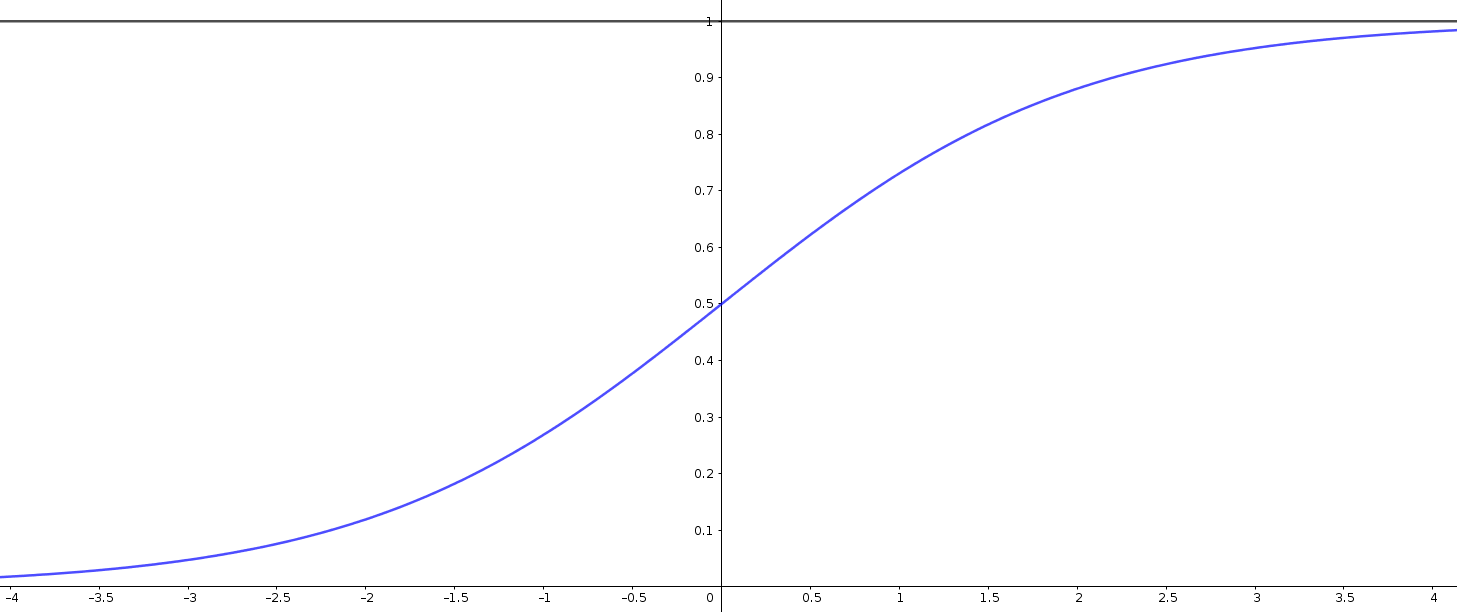
\includegraphics[width=0.65\textwidth]{images/logistica.png}
    \caption{La función logística.} \label{fig:funcion_logistica}
\end{figure}

Supongamos el conjunto de datos $\mathcal{X} = \{x_1,\dots,x_N\} \subset \R^d$, con correspondientes etiquetas $y_1,\dots,y_N$. En LDML, la función logística se utiliza para definir una probabilidad, la cual asignará a pares de puntos una probabilidad mayor conforme menor sea la distancia entre ellos. Para medir la distancia, LDML utilizará una matriz de métrica $M$ semidefinida positiva, quedando la expresión de la probabilidad como
\begin{equation}
    p_{ij,M} = \sigma(b - \|x_i-x_j\|_M^2),
\end{equation} 

donde $b$ es un valor umbral positivo que determinará el valor máximo alcanzable por la función logística, y que puede ser estimado mediante validación cruzada. Asociada a esta probabilidad podemos definir una variable aleatoria que sigue una distribución de Bernouilli, y que toma los valores 0 y 1, según el par $(x_i,x_j)$ pertenezca o no a la misma clase. Dicha distribución viene determinada por la función masa de probabilidad
\[ f_{ij,M}(x) = (p_{ij,M})^{x}(1-p_{ij,M})^{1-x}, \quad x  \in \{0,1\}. \]

La función que busca maximizar la técnica LDML es el logaritmo de la verosimilitud de la distribución anterior para el conjunto de datos dado, esto es,
\begin{equation}
    \mathcal{L}(M) = \sum_{i,j=1}^N y_{ij}\log p_{ij,M} + (1-y_{ij})\log(1-p_{ij,M}),
\end{equation}

donde $y_{ij}$ es una variable binaria que toma el valor 1 si $y_i = y_j$, y 0 en caso contrario. Esta función es diferenciable, cóncava (es una combinación positiva de funciones que se pueden expresar como un menos logaritmo de suma de exponenciales, que son cóncavos) y está mayorada, luego tenemos la garantía de poder alcanzar un máximo global. Teniendo en cuenta que, si $x_{ij} \equiv (x_i-x_j)^T(x_i-x_j)$ y $p_{ij} \equiv p_{ij,M}$, y por las propiedades de la derivada de la función logística su gradiente presenta la expresión
\begin{align*}
    \mathcal{\nabla L}(M) &= \sum_{i,j=1}^N y_{ij}\frac{-x_{ij} p_{ij}(1 - p_{ij})}{p_{ij}} + (1-y_{ij})\frac{x_{ij}p_{ij}(1-p_{ij})}{1-p_{ij}} \\
                          &= \sum_{i,j=1}^N -y_{ij}x_{ij}(1 - p_{ij}) + (1-y_{ij})x_{ij}p_{ij} \\
                          &= \sum_{i,j=1}^N x_{ij}((1-y_{ij})p_{ij}-(1-p_{ij})y_{ij}) \\
                          &= \sum_{i,j=1}^N x_{ij}(p_{ij}-y_{ij}),
\end{align*}

los métodos iterativos de gradiente ascendente combinados con proyecciones sobre el cono de las matrices semidefinidas positivas, conforman el algoritmo de programación semidefinida que es utilizado en LDML para la obtención de la métrica que optimiza su función objetivo.

%% *** Imagen de la funcion logistica



\section{El kernel trick. Algoritmos de aprendizaje de métricas de distancia basados en kernels}

\subsection{El kernel trick}

Los métodos de kernel conforman un paradigma dentro del aprendizaje automático que resulta de gran utilidad en muchos de los problemas que se abordan en esta disciplina. Normalmente surgen en problemas en los que el algoritmo de aprendizaje ve mermada su capacidad, generalmente, debido a la forma del conjunto de datos. Esto ocurre, por ejemplo, en las máquinas de vectores soporte. Aunque no vamos a entrar en los detalles de este algoritmo, nos va a servir para ilustrar la necesidad de los métodos de kernel en el aprendizaje automático.

Las \emph{máquinas de vectores soporte} (SVM, \emph{Support Vector Machines}) son un modelo de clasificación lineal binario que, en su versión más sencilla, cuando los datos son separables, busca establecer el hiperplano que mejor que mejor separa los datos, esto es, aquel para el cual se maximiza la distancia (margen) a los conjuntos que determinan cada clase. Los puntos de ambos conjuntos donde se materializa dicho margen son los denominados \emph{vectores soporte}. En la figura \ref{fig:svm_ejemplo} se muestra cómo actúa este clasificador.

\begin{figure}[h]
    \centering
    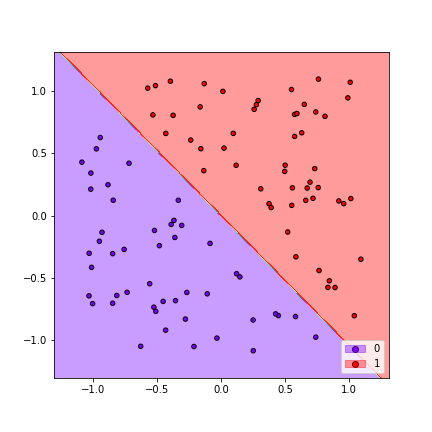
\includegraphics[width=0.5\textwidth]{images/svm_example.png}
    \caption{Clasificación realizada por las máquinas de vectores soporte en su versión básica.} \label{fig:svm_ejemplo}
\end{figure} 

Sin embargo, en muchas ocasiones, aunque los datos sean visiblemente separables, puede resultar imposible separarlos mediante un hiperplano, como sucede en el ejemplo de la figura \ref{fig:svm_ejemplo2}. En ella, se ha considerado un subconjunto finito $\mathcal{X}$ de números reales, de forma que a aquellos $x \in \mathcal{X}$ con $|x| > 1$ se les ha asignado la clase $1$ y a aquellos con $|x| \le 1$ la clase $-1$. Es inmediato observar que, aunque las regiones de las dos clases están claramente diferenciadas, no es posible separarlas mediante un hiperplano.

\begin{figure}[h]
    \centering
    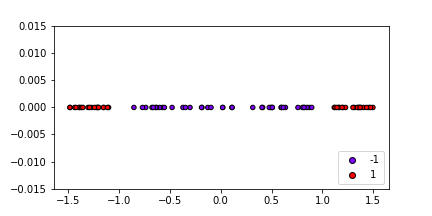
\includegraphics[width=0.5\textwidth]{images/svm_problem.png}
    \caption{Conjunto de datos para el que SVM no puede establecer un hiperplano separador.} \label{fig:svm_ejemplo2}
\end{figure} 

A pesar de esto, es posible establecer una transformación en los datos que los incluya en un espacio de dimensión mayor en el cual los datos sí sean separables mediante hiperplanos. En efecto, si definimos la aplicación $\phi\colon \R \to \R^2$ por $\phi(x) = (x,x^2)$, los datos de $\phi(\mathcal{X})$ sí que son separables en $\R^2$. Concretamente, podemos tomar el hiperplano $H = \{(x,y) \in \R^2 \colon y = 1\}$ como hiperplano separador. Esta misma idea podemos utilizarla sobre SVM: transformamos los datos y aplicamos el algoritmo en el espacio transformado obteniendo el hiperplano. Si después queremos predecir la clase de un nuevo dato, podemos aplicarle la transformación y asignarle la clase según el lado del hiperplano en el que ha caído. La figura \ref{fig:svm_ejemplo3} muestra el resultado de aplicar SVM en el espacio transformado sobre el ejemplo dado.

\begin{figure}[h]
    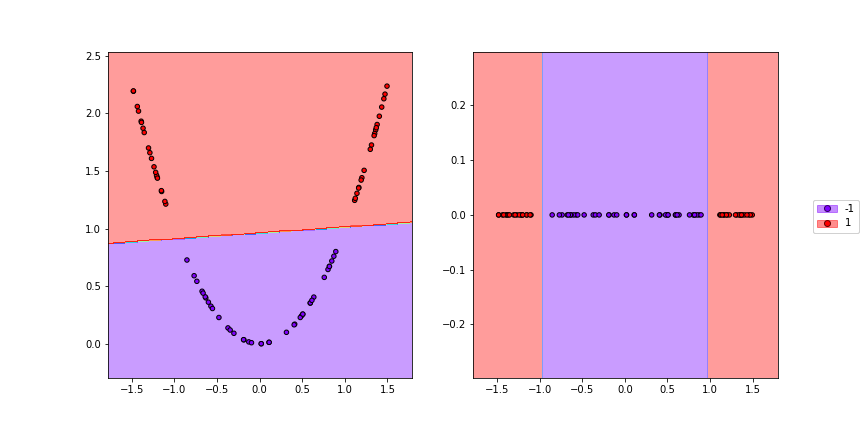
\includegraphics[width=0.8\textwidth]{images/svm_solution.png}
    \centering
    \caption{Resolución mediante máquinas de vectores soporte del problema de la figura \ref{fig:svm_ejemplo2} en el espacio de características. A la derecha se muestra el efecto del clasificador aprendido en el espacio de características sobre el conjunto de datos original.} \label{fig:svm_ejemplo3}
\end{figure} 

En general, cuando nos encontramos con este tipo de problemas siempre podemos enviar los datos a un nuevo espacio de dimensión mayor, definiendo una aplicación $\phi\colon \mathcal{X} \to \mathcal{F}$. El espacio $\mathcal{F}$ lo tomamos como espacio de Hilbert y recibe el nombre de \emph{espacio de características}. Aunque con el ejemplo anterior hemos podido comprobar el potencial de esta herramienta, tiene un gran inconveniente, y es que enviar los datos a un espacio de características puede aumentar en gran medida la dimensión del problema, y por lo tanto la aplicación de los algoritmos en el espacio de características puede ser muy costoso computacionalmente. Además, si quisiéramos trabajar en espacios de características de dimensión infinita sería imposible tratar los datos computacionalmente de esta forma. Para solventar estos problemas surge el concepto de \emph{kernel trick}.

Si $\phi\colon \mathcal{X} \to \mathcal{F}$ es la aplicación de envío al espacio de características, se define la \emph{función kernel} asociada como la forma bilineal simétrica $K \colon \mathcal{X} \times \mathcal{X} \to \R$ que determina los productos escalares de los datos en el espacio de características, esto es,
$K(x,x') = \langle \phi(x), \phi(x') \rangle$. La clave del éxito de las funciones kernel es que, en muchos algoritmos, como ocurre en el caso de SVM, no es necesario tratar con los valores de los datos, sino únicamente con los productos escalares entre ellos. Por tanto, conociendo la función kernel disponemos de la información necesaria para trabajar en el espacio de características, sea cual sea su dimensión. Notemos por último que, si $X = \{x_1,\dots,x_N\}$, el tamaño, la función kernel puede verse como una matriz $K \in S_N(\R)$ donde $K_{ij} = \langle \phi(x_i), \phi(x_j) \rangle$, por lo que la complejidad del problema va a depender únicamente del tamaño del conjunto de datos, independientemente de la dimensión del espacio de características.

A continuación vamos a ver algunas de las funciones kernel más utilizadas. Con ellas podremos observar también cómo es posible utilizar las funciones kernel para trabajar en espacios de dimensión infinita.

\begin{ex}[El kernel lineal]
    El kernel lineal es el caso más sencillo de kernel, y viene representado por la función
    \[ K(x,x') = \langle x, x' \rangle. \]
    Se corresponde con la transformación identidad sobre el mismo espacio de partida.
\end{ex}

\begin{ex}[Kernels polinómicos]
    Los kernels polinómicos de grado $k$ vienen dados por funciones kernel de la forma
    \[ K(x,x') = (\gamma \langle x,x' \rangle + c_0)^k. \]
    Fijado $k \in \N$, veamos que en efecto $K$ es una función kernel, es decir, que hay una transformación $\phi$ para la cual $K(x,x') = \langle \phi(x),\phi(x') \rangle$. Supongamos $\gamma = c_0 = 1$ (los cálculos son análogos para cualquier valor de estos parámetros). Además, supongamos $x = (x_1,\dots,x_d), x' = (x'_1,\dots,x'_d)$ y notamos $x_0 = x'_0 = 1$. Utilizamos tambiénla notación multiíndice de los polinomios en varias variables, de forma que si $\alpha = (\alpha_1,\dots,\alpha_d) \in (\N\cup\{0\})^d$, la expresión $x_{\alpha}$ representa el monomio $x_{\alpha_1}\dots x_{\alpha_d}$. Entonces se tiene
    \begin{equation*}
        K(x,x') = \prod_{i=1}^k (1 + \langle x, x' \rangle) 
                = \prod_{i=1}^k \sum_{j=0}^d x_jx_j' 
                = \sum_{\alpha \in \{0,\dots,d\}^k} x_{\alpha} x_{\alpha}'
    \end{equation*}
    Si ahora definimos la aplicación $\phi \colon \R^d \to \R^{(d+1)^k}$ como
    \[\phi(x) = (x_{(0,\dots,0)},x_{(0,\dots,1)},\dots,x_{(0,\dots,n)},x_{(0,\dots,1,0)},\dots,x_{(n,\dots,n)}),\]
    se concluye que 
    \[ \langle \phi(x), \phi(x') \rangle = \sum_{\alpha \in \{0,\dots,d\}^k} x_{\alpha} x_{\alpha}' = K(x,x'). \]
    Por tanto, $K$ es una función kernel y está construida a partir de transformaciones polinómicas de grado máximo $k$.
\end{ex}

\begin{ex}[El kernel gaussiano]
    El kernel gaussiano viene determinado por la aplicación $K\colon \mathcal{X} \times \mathcal{X} \to \R$ dada por
    \[ K(x,x') = \exp(-\gamma\|x-x'\|^2).\]
    Es el kernel más popular junto al polinómico. También se le conoce como kernel RBF (\emph{Radial Basis Funcion}), pues las funciones que definen los productos escalares dependen únicamente de la distancia entre los datos.

    Veamos que, efectivamente, $K$ es una función kernel y que el espacio de características tiene dimensión infinita. Supongamos, por simplicidad, que el espacio de partida es $\R$. Entonces,
    \begin{align*}
        K(x,x') &= e^{-\gamma(x-x')^2} = e^{-\gamma x^2 + 2\gamma xx' -\gamma x'^2 } \\
                &= e^{-\gamma x^2 -\gamma x'^2 }e^{2\gamma xx'} \\
                &= e^{-\gamma x^2 -\gamma x'^2 }\sum_{n=0}^{\infty} \frac{(2\gamma xx')^n}{n!} \\
                &= e^{-\gamma x^2 -\gamma x'^2 }\sum_{n=0}^{\infty} \sqrt{\frac{2\gamma}{n!}}x^n\sqrt{\frac{2\gamma}{n!}}x'^n \\
                &= \langle \phi(x), \phi(x') \rangle_{l_2}, 
    \end{align*}

    donde $l_2$ es el espacio de Hilbert las sucesiones de cuadrado sumables y $\phi \colon \R \to l_2$ es la aplicación dada por
    \[\phi(x) = e^{-\gamma x^2}\left\{ \sqrt{\frac{2\gamma}{n!}}x^n \right\}_{n=0}^{\infty}.\]
    Notemos que $\phi$ está bien definida, pues la sucesión que define tiene como suma de cuadrados una exponencial. Por tanto, con el kernel gaussiano obtenemos un espacio de características de dimensión infinita.
\end{ex}

\begin{ex}[Otros kernels]
    $ $ \newline
    \begin{enumerate}
        \item Kernel laplaciano: \[ K(x,x') = \exp(-\gamma\|x-x'\|_1). \]
        \item Kernel sigmoidal: \[ K(x,x') = \tanh(\gamma \langle x,x' \rangle + c_0). \]
        \item Kernel cosenoidal: \[ K(x,x') = \frac{\langle x,x' \rangle}{ \|x\|\|x'\|}. \]
    \end{enumerate}
    En general, toda matriz semidefinida positiva es la matriz de una función kernel. Recíprocamente, las matrices de las funciones kernel son siempre semidefinidas positivas.
\end{ex}

En el aprendizaje de métricas de distancia, la utilidad de los kernels se debe a las limitaciones que vienen dadas por las distancias de Mahalanobis aprendidas. Aunque las métricas aprendidas pueden utilizarse posteriormente para aprender mediante clasificadores no lineales, como el kNN, las métricas en sí hemos visto que vienen determinadas por una aplicación lineal. Estas siempre vienen determinadas por la imagen de una base de vectores en el espacio de partida, lo que condiciona a que en la transformación resultante del aprendizaje se tenga la libertad únicamente de elegir las imágenes de tantos datos como dimensión tenga el espacio, transformando el resto de vectores por linealidad. Cuando la cantidad de datos es mucho mayor que la dimensión de su espacio esto puede convertirse en una limitación.

El uso de las funciones kernel es factible en muchos de los algoritmos del aprendizaje de métricas de distancia gracias a que, como ocurría con las máquinas de vectores soporte, muchos de estos algoritmos solo necesitan tratar con los productos escalares entre los datos, en lugar de hacerlo directamente con los datos. A modo de ejemplo, vamos a ver que es posible calcular distancias euclídeas, una herramienta esencial en muchos de los algoritmos, en el espacio de características, utilizando únicamente productos escalares entre los datos. En efecto, si $K$ es la matriz de la función kernel, $\phi\colon \mathcal{X} \to \mathcal{F}$ es la transformación al espacio de características y $x_i,x_j \in \mathcal{X}$, se tiene
\begin{equation} \label{eq:dist_features}
    \begin{split}
    \|\phi(x_i)-\phi(x_j)\|^2 &= \langle \phi(x_i)-\phi(x_j), \phi(x_i) - \phi(x_j) \rangle \\
                              &= \langle \phi(x_i),\phi(x_i) \rangle - 2 \langle\phi(x_i), \phi(x_j) \rangle + \langle \phi(x_j), \phi(x_j) \rangle \\
                              &= K_{ii} + K_{jj} -2K_{ij}.
    \end{split}
\end{equation}

El siguiente problema común a todos los algoritmos de aprendizaje de métricas basados en kernels consiste en cómo tratar la transformación aprendida. En este caso, el aprendizaje consistirá en aprender una aplicación lineal en el espacio de características $L \colon \mathcal{F} \to \R^d$ que, como ocurre en los algoritmos ya estudiados, inducirá una distancia en el espacio de destino. El problema en esta situación es que $\mathcal{F}$ podría ser de muy alta dimensionalidad, o incluso de dimensión infinita, luego $L$ podría no ser tratable matricialmente. Retomando el ejemplo de las máquinas de vectores soporte, surge un problema similar, pues el hiperplano aprendido puede representarse mediante un vector $w$, que de nuevo podría tener dimensión muy alta o infinita. En este caso, se conocen \emph{teoremas de representación} que permiten expresar $w$ como combinación lineal de los datos en el espacio de características, y dicha combinación lineal permite utilizar las funciones kernel para la transformación.

En el aprendizaje de métricas de distancia, si suponemos la aplicación lineal que queremos aprender $L$ también continua (es decir, $L \in \mathcal{L}(\mathcal{F},\R^d)$), podemos expresarla como un vector de funcionales lineales y continuos, los cuales, por el teorema de representación de Riesz, están determinados por el producto escalar por un determinado vector, es decir, $L = (\langle \cdot, w_1 \rangle, \dots, \langle \cdot , w_d \rangle)$. Para los algoritmos que vamos a estudiar, se conocen diversos teoremas de representación \cite{neurocomputing,hofmann2008kernel,kda,dmlmj,kpca} que permiten expresar los vectores $w_i$ como combinación lineal de los datos en el espacio de características, esto es, para cada $i \in \{1,\dots,d'\}$ existe un vector $\alpha^i = (\alpha_1^i,\dots,\alpha_{N}^i) \in \R^{N}$ tal que $w_i = \sum_{j=1}^N \alpha_j^i \phi(x_j)$. En consecuencia, se verifica que
\[L\phi(x) = A \begin{pmatrix} K(x_1,x) \\ \vdots \\ K(x_N,x) \end{pmatrix},\]
donde $A \in \mathcal{M}_{d'\times N}(\R)$ viene dada por $A_{ij} = \alpha_j^i$.

\begin{comment}
Vamos a ver que en el aprendizaje de métricas de distancia podemos seguir el mismo planteamiento, gracias al teorema que se enuncia a continuación.
\end{comment}

\begin{comment}
\begin{thm}[Teorema de representación para el aprendizaje de métricas de distancia] \label{thm:representer}
    Sea $\mathcal{X} = \{x_1,\dots,x_N\} \subset \R^d$, $\mathcal{F}$ un espacio de Hilbert de características, y $\phi \colon \mathcal{X} \to \mathcal{F}$ una aplicación. Consideramos también la función kernel $K \colon \R^d \times \R^d \to \R$. Sean $d' \le d$ y $L\colon \mathcal{F} \to \R^{d'}$ una aplicación lineal y continua. Entonces, podemos escribir $L = (L_1, \dots, L_{d'})$, donde $L_i \colon \mathcal{F} \to \R$ viene dado por $L_i(u) = \langle w_i, u \rangle$ para todo $u \in \mathcal{F}$. Supongamos que $L$ verifica alguna de las siguientes condiciones:

    \begin{enumerate}
        \item  $w_i$ es un vector propio de un operador autoadjunto que es combinación lineal de productos tensoriales de la forma $\phi(x_i)-\phi(x_j)$ consigo mismos, para cada $i = \{1,\dots,d'\}$. \label{item:representer:1}
        \item Si notamos $D_{ij}(L) = \|L(\phi(x_i) - \phi(x_j))\|^2$, para $i,j = 1,\dots,N$, $L$ es solución de un problema de la forma
        \begin{equation}
            \min_{L} f(D_{11}(L),D_{12}(L),\dots,D_{1N}(L),D_{21}(L),\dots,D_{2N}(L),\dots,D_{NN}(L))
        \end{equation} \label{item:representer:2}
    \end{enumerate}

    Entonces, para cada $i \in \{1,\dots,d'\}$ existe un vector $\alpha^i = (\alpha_1^i,\dots,\alpha_{N}^i) \in \R^{N}$ tal que $w_i = \sum_{j=1}^N \alpha_j^i \phi(x_j)$.

    En consecuencia, se verifica que 
    \[L\phi(x) = A \begin{pmatrix} K(x_1,x) \\ \vdots \\ K(x_N,x) \end{pmatrix},\]
    donde $A \in \mathcal{M}_{d'\times N}(\R)$ viene dada por $A_{ij} = \alpha_j^i$  .
\end{thm}
\end{comment}

Gracias a estos teoremas, podemos tratar el problema computacionalmente si somos capaces de calcular los coeficientes de la matriz $A$. A la hora de transformar los datos de $\mathcal{X}$ bastará con multiplicar $A$ por la columna adecuada de la matriz del kernel. Si queremos transformar nuevos datos podemos de la misma forma definir una matriz (en este caso, no necesariamente cuadrada) con los productos escalares entre los datos de entrenamiento y los nuevos datos. De nuevo, escogiendo la columna adecuada en dicha matriz podremos transformar los datos según la aplicación definida por $L$.

Cada técnica de aprendizaje de métricas que admita el uso de kernels utilizará herramientas distintas para su funcionamiento, cada una de ellas basada en los algoritmos originales. En las siguientes secciones se describirán las kernelizaciones de algunos de los algoritmos estudiados.


\subsection{KLMNN}

KLMNN \cite{klmnn} es la versión kernelizada de LMNN. En ella, los datos del conjunto $\mathcal{X}$ se envían al espacio de características para aprender en dicho espacio una distancia que minimice la función de error establecida en el problema de LMNN.

Aunque el problema formulado en la versión no kernelizada se realizó respecto a una matriz de métrica $M$, mediante la función de error \ref{eq:lmnn:M}, a la hora de trabajar en espacios de características nos interesará más trabajar con una aplicación lineal, aunque se pierda la convexidad del problema, para poder utilizar el teorema de representación. Por tanto, adaptando al espacio de características la función de error propuesta en \ref{eq:lmnn:L}, el problema formulado para la versión kernelizada consiste en
\begin{equation} \label{eq:klmnn:L}
\begin{split}
    \min_{L\in \mathcal{L}(\mathcal{F},\R^{d})} \quad \varepsilon(L) &= (1-\mu)\sum_{i=1}^N\sum_{j \istargetof i} \|L(\phi(x_i) - \phi(x_j))\|^2 \\
                &+ \mu \sum_{i=1}^N\sum_{j \istargetof i} \sum_{l=1}^N(1-y_{il})[1 + \|L(\phi(x_i) - \phi(x_j))\|^2-\|L(\phi(x_i) - \phi(x_l))\|^2]_+. 
 \end{split}
\end{equation}

Como consecuencia del teorema de representación, se verifica que, para cada $x_i \in \mathcal{X}$, $L\phi(x_i) = AK_{.i}$, donde $A \in \mathcal{M}_{d' \times N}(\R)$ es la matriz dada por el teorema de representación, y $K_{.i}$ es la $i$-ésima columna de la matriz de kernel. Utilizando esto en la expresión del error, obtenemos
\begin{align*}
& (1-\mu)\sum_{i=1}^N\sum_{j \istargetof i} \|L(\phi(x_i) - \phi(x_j))\|^2 
                + \mu \sum_{i=1}^N\sum_{j \istargetof i} \sum_{l=1}^N(1-y_{il})[1 + \|L(\phi(x_i) - \phi(x_j))\|^2-\|L(\phi(x_i) - \phi(x_l))\|^2]_+ \\
&= (1-\mu)\sum_{i=1}^N\sum_{j \istargetof i} \|A(K_{.i} - K_{.j})\|^2 
                + \mu \sum_{i=1}^N\sum_{j \istargetof i} \sum_{l=1}^N(1-y_{il})[1 + \|A(K_{.i} - K_{.j})\|^2-\|A(K_{.i} - K_{.l})\|^2]_+.
 \end{align*}

La expresión anterior depende únicamente de $A$ y de las funciones kernel, y minimizándola como función en $A$ (la notamos $\varepsilon(A)$) obtenemos el mismo valor que al minimizar $\varepsilon(L)$. Observemos también que la expresión $\varepsilon(A)$ requiere el cálculo de los vecinos objetivo y los impostores, pero estos dependen únicamente de las distancias en el espacio de características, las cuales ya hemos visto que son calculables, como se indica en la igualdad \ref{eq:dist_features}. Por tanto, todos los aspectos de $\varepsilon(A)$ son tratables computacionalmente, así que si aplicamos métodos de gradiente sobre $\varepsilon(A)$ podremos reducir el valor de la función objetivo, siempre teniendo en cuenta que podemos quedar atrapados en óptimos locales, pues el problema no es convexo. Finalmente, una vez encontrada una matriz $A$ que minimiza $\varepsilon(A)$, tendremos determinada la aplicación $L$ asociada gracias al teorema de representación, y podemos usar $A$ junto con las funciones kernel para transformar nuevos datos. 

\begin{comment}
Concluimos viendo la expresión de un subgradiente $G \in \partial\varepsilon/\partial A$ de $\varepsilon(A)$.

$G = $
\end{comment}

\subsection{KANMM}

KANMM \cite{anmm} es la versión kernelizada de ANMM. En ella, los datos del conjunto $\mathcal{X}$ se envían al espacio de características mediante la aplicación $\phi\colon \mathcal{X} \to \mathcal{F}$. En dicho espacio aplicamos ANMM para obtener la aplicación lineal buscada.

Recordamos que el primer paso necesario para la aplicación de ANMM era la obtención de los vecindarios homogéneo y heterogéneo para cada dato $x_i \in \mathcal{X}$. Observemos que para este cálculo únicamente es necesario comparar distancias en el espacio de características, lo cual hemos visto que se puede realizar gracias a la función kernel, mediante la igualdad \ref{eq:dist_features}. Notaremos a los vecindarios en el espacio de características como $N_{\phi(x_i)}^o$ y $N_{\phi(x_i)}^e$, respectivamente, para cada $x_i$.

Las matrices (o endomorfismos, más en general) de dispersión y compacidad en el espacio de características vienen dados por
\begin{align*}
    S^{\phi} = \sum\limits_{i,k \colon \phi(x_k) \in N_{\phi(x_i)}^e} \frac{(\phi(x_i)-\phi(x_k))(\phi(x_i)-\phi(x_k))^T}{|N_{\phi(x_i)}^e|} \\
    C^{\phi} = \sum\limits_{i,j \colon \phi(x_j) \in N_{\phi(x_i)}^o} \frac{(\phi(x_i)-\phi(x_j))(\phi(x_i)-\phi(x_j))^T}{|N_{\phi(x_i)}^o|}.
\end{align*}

El problema a optimizar se expresa, por tanto, como
\begin{equation}
\begin{split}
    \max_{L \in \mathcal{L}(\mathcal{F},\R^{d'})} &\quad \tr\left(L(S^{\phi}-C^{\phi})L^T\right)  \\
    \text{s.a.: } &\quad LL^T = I
\end{split}
\end{equation}
De acuerdo con los teoremas de representación, cada uno de los vectores $w_i, i = 1,\dots,d'$ de $\mathcal{F}$ que caracterizan $L$ verifican $w_i = \sum_{j=1}^N \alpha_j^i \phi(x_j)$. En consecuencia, $L\phi(x_i) = AK_{.i}$, donde $A$ es la matriz de coeficientes del teorema de representación y $K_{.i}$ representa la $i$-ésima columna de la matriz del kernel. Entonces,
\begin{equation*}
    \begin{split}
        L(\phi(x_i)-\phi(x_j))(\phi(x_i)-\phi(x_j))^TL^T = A(K_{.i}-K_{.j})(K_{.i}-K_{.j})^TA^T,
    \end{split}
\end{equation*}
y si consideramos las matrices
\begin{align*}
    \widetilde{S}^{\phi} = \sum\limits_{i,k \colon \phi(x_k) \in N_{\phi(x_i)}^e} \frac{(K_{.i}-K_{.k})(K_{.i}-K_{.k})^T}{|N_{\phi(x_i)}^e|} \\
    \widetilde{C}^{\phi} = \sum\limits_{i,j \colon \phi(x_j) \in N_{\phi(x_i)}^o} \frac{(K_{.i}-K_{.j})(K_{.i}-K_{.j})^T}{|N_{\phi(x_i)}^o|},
\end{align*}
se cumple que el margen promedio viene dado por
\begin{equation*}
    \gamma^L = \tr(L(S^{\phi}-C^{\phi})L^T) = \tr(LS^{\phi}L^T-LC^{\phi}L^T) = \tr(A \widetilde{S}^{\phi} A^T - A\widetilde{C}^{\phi}A^T = \tr(A(\widetilde{S}^{\phi}-\widetilde{C}^{\phi})A^T))
\end{equation*} 

Si imponemos la restricción $AA^T = I$, el teorema \ref{thm:eigen_trace_opt} nos dice de nuevo que podemos tomar como matriz $A$ aquella que contenga por filas los vectores propios de $\widetilde{S}^{\phi}-\widetilde{C}^{\phi}$ asociados a sus $d'$ valores propios. Observemos que ambas matrices podemos calcularlas a partir de la función kernel, y la matriz $A$ así obtenida determina la aplicación lineal, por el teorema de representación. Por tanto, hemos obtenido finalmente un método basado en kernels para la aplicación de ANMM en espacios de características.

\subsection{KDMLMJ}

KDMLMJ \cite{dmlmj} es la versión kernelizada de DMLMJ. En ella, los datos del conjunto $\mathcal{X}$ se envían al espacio de características mediante la aplicación $\phi\colon \mathcal{X} \to \mathcal{F}$, en el cual se aplica DMLMJ para obtener una aplicación lineal.

De nuevo, es posible calcular los vecindarios $k$-positivo y $k$-negativo $V_k^+(\phi(x_i))$ y $V_k^-(\phi(x_i))$ para cada $x_i \in \mathcal{X}$ gracias a la igualdad \ref{eq:dist_features}. No ocurre lo mismo con los endomorfismos asociadas a los espacios de diferencias,
\begin{align*}
    \Sigma_S^{\phi} &= \frac{1}{|S|}\sum_{i=1}^{N} \left[ \sum_{\phi(x_j) \in V_k^+(\phi(x_i))} (\phi(x_i)-\phi(x_j))(\phi(x_i)-\phi(x_j))^T\right] \\
    \Sigma_D^{\phi} &= \frac{1}{|D|}\sum_{i=1}^{N} \left[ \sum_{\phi(x_j) \in V_k^-(\phi(x_i))} (\phi(x_i)-\phi(x_j))(\phi(x_i)-\phi(x_j))^T\right].
\end{align*}
El problema de optimización viene dado por
\[ \max_{L \in \mathcal{L}(\mathcal{F}, \R^{d'})} \quad J(L) =  \tr\left( (L\Sigma_S^{\phi} L^T)^{-1} (L\Sigma_D^{\phi} L^T) + (L \Sigma_D^{\phi} L^T)^{-1} (L \Sigma_S^{\phi} L^T) \right).\]
 De nuevo se tiene, por los teoremas de representación, que $L\phi(x_i) = AK_{.i}$ para cada $x_i \in \mathcal{X}$, donde $A$ es la matriz del teorema de representación y $K_{.i}$ es la $i$-ésima columna de la matriz de kernel. Si, razonando como en la sección anterior, definimos las matrices
\begin{align*}
    U &= \frac{1}{|S|}\sum_{i=1}^{N} \left[ \sum_{\phi(x_j) \in V_k^+(\phi(x_i))} (K_{.i}-K_{.j})(K_{.i}-K_{.j})^T\right] \\
    V &= \frac{1}{|D|}\sum_{i=1}^{N} \left[ \sum_{\phi(x_j) \in V_k^-(\phi(x_i))} (K_{.i}-K_{.j})(K_{.i}-K_{.j})^T\right],
\end{align*}
obtenemos que
\begin{equation*}
    \begin{split}
        \tr\left( (L\Sigma_S^{\phi} L^T)^{-1} (L\Sigma_D^{\phi} L^T) + (L \Sigma_D^{\phi} L^T)^{-1} (L \Sigma_S^{\phi} L^T) \right) = \\
        \tr\left( (AUA^T)^{-1} (AV A^T) + (A V A^T)^{-1} (A U A^T) \right).
    \end{split}
\end{equation*}
De forma análoga a DMLMJ, podemos encontrar una matriz $A$ que maximice esta última igualdad tomando los vectores propios de $U^{-1}V$ para los que se maximice el valor $\lambda + 1 /\lambda$, donde $\lambda$ es el valor propio asociado. Como las matrices $U$ y $V$ se pueden obtener a partir de la función kernel, y $A$ determina a $L$ por el teorema de representación, hemos obtenido un algoritmo para la aplicación de DMLMJ en el espacio de características.


\subsection{KDA}

KDA (\emph{Kernel Discriminant Analysis}) \cite{kda} es la versión kernelizada del análisis discriminante lineal. La kernelización de este algoritmo permitirá encontrar direcciones no lineales que separen bien a los datos de acuerdo con el criterio establecido en el análisis discriminante. Una vez más, enviamos los datos del conjunto $\mathcal{X}$ al espacio de características mediante la aplicación $\phi \colon \mathcal{X} \to \mathcal{F}$. Sobre dicho espacio aplicaremos el análisis discriminante lineal.

Supongamos, al igual que en LDA, que el conjunto de posibles clases es $\mathcal{C}$, de cardinal $r$, y para cada $c \in \mathcal{C}$ definimos $\mathcal{C}_c = \{i \in \{1,\dots,N\} \colon y_i = c\}$ y $N_c = |\mathcal{C}_c|$, con $\mu_c^{\phi}$ el vector media de la clase $c$ y $\mu^{\phi}$ el vector media de todos los datos, considerándolos dentro del espacio de características. El problema que buscamos resolver en este caso es
\begin{equation} \label{eq:kda}
    \max_{\substack{L \in \mathcal{L}(\mathcal{F}, \R^{d'}) }} \quad \tr\left(\frac{L S_b^{\phi} L^T}{LS_w^{\phi}L^T}\right),
\end{equation}
donde $S_b^{\phi}$ y $S_w^{\phi}$ son los operadores que miden la dispersión entre clases e intra-clase, respectivamente, y vienen dados por

\begin{align*}
    S_b^{\phi} &= \sum_{c \in \mathcal{C}}(\mu_c^{\phi} - \mu^{\phi})(\mu_c^{\phi} - \mu^{\phi})^T \\
    S_w^{\phi} &= \sum_{c \in \mathcal{C}}\sum_{i \in \mathcal{C}_c}(\phi(x_i)-\mu_c^{\phi})(\phi(x_i)-\mu_c^{\phi})^T,
\end{align*}

De nuevo hacemos uso de los teoremas de representación, de forma que si $L = (\langle w_1,\cdot\rangle, \dots, \langle w_{d'}, \cdot \rangle)$, se verifica que $w_i = \sum_{j=1}^N \alpha_j^i \phi(x_j)$ para cada $i = 1,\dots,d'$ y
\[L\phi(x) = A \begin{pmatrix} K(x_1,x) \\ \vdots \\ K(x_N,x) \end{pmatrix}, \]
para los coeficientes $\alpha_j^i$ y la matriz $A$ en las condiciones del teorema de representación. Vamos a buscar de nuevo una expresión del problema \ref{eq:kda} que dependa únicamente de la función kernel y de la matriz $A$. Para ello, observemos que para los vectores media de cada clase se verifica
\[ L\mu_c^{\phi} = L\left(\frac{1}{N_c} \sum_{i \in \mathcal{C}_c} \phi(x_i)\right) = \frac{1}{N_c}\sum_{i \in \mathcal{C}_c}L\phi(x_i) = \frac{1}{N_c}\sum_{i \in \mathcal{C}_c}AK_{.i},  \]
donde $K_{.i}$ es la columna $i$-ésima de la matriz kernel. Análogamente, para el vector media global, se tiene
\[ L\mu^{\phi} = \frac{1}{N} \sum_{i=1}^NAK_{.i}. \]

En consecuencia,
\begin{align*}
    L(\mu_c^{\phi} - \mu^{\phi})(\mu_c^{\phi} - \mu^{\phi})^TL^T &= (L\mu_c^{\phi} - L\mu^{\phi})(L\mu_c^{\phi} - L\mu^{\phi})^T \\
                                     &=  \left( \frac{1}{N_c}\sum_{i \in \mathcal{C}_c} AK_{.i} - \frac{1}{N}\sum_{i=1}^N AK_{.i} \right)\left( \frac{1}{N_c}\sum_{i \in \mathcal{C}_c} AK_{.i} - \frac{1}{N}\sum_{i=1}^N AK_{.i} \right)^T.
\end{align*}
Notemos que la última expresión depende únicamente de $A$ y de la función kernel. Por otra parte, para $x_i \in \mathcal{X}$ con $y_i = c$ se tiene
\begin{multline*}
    L(\phi(x_i) - \mu_c^{\phi})(\phi(x_i) - \mu_c^{\phi})^TL^T = (L\phi(x_i) - L\mu_c^{\phi})(L\phi(x_i) - L\mu_c^{\phi})^T \\
                                     = \left(AK_{.i} - \frac{1}{N_c}\sum_{j \in \mathcal{C}_c} AK_{.j} \right)\left(AK_{.i} - \frac{1}{N_c}\sum_{j \in \mathcal{C}_c} AK_{.j} \right)^T \\
                                     = \left(AK_{.i} - \frac{1}{N_c}\sum_{j \in \mathcal{C}_c} AK_{.j} \right)\left(K_{.i}^TA^T - \frac{1}{N_c}\sum_{j \in \mathcal{C}_c} K_{.j}^TA^T \right) \\
                                     = AK_{.i}K_{.i}^TA^T - \frac{1}{N_c}\sum_{j\in \mathcal{C}_c}AK_{.i}K_{.j}^TA^T - \frac{1}{N_c}\sum_{j\in \mathcal{C}_c}AK_{.j}K_{.i}^TA^T + \frac{1}{N_c^2}\sum_{j \in \mathcal{C}_c}\sum_{l \in \mathcal{C}_c}AK_{.j}K_{.l}^TA^T.
\end{multline*}
Sumando en $i \in \mathcal{C}_c$ obtenemos
\begin{multline*}
    \sum_{i\in\mathcal{C}_c}L(\phi(x_i) - \mu_c^{\phi})(\phi(x_i) - \mu_c^{\phi})^TL^T \\
    = \sum_{i \in \mathcal{C}_c}\left[AK_{.i}K_{.i}^TA^T - \frac{1}{N_c}\sum_{j\in \mathcal{C}_c}AK_{.i}K_{.j}^TA^T - \frac{1}{N_c}\sum_{j\in \mathcal{C}_c}AK_{.j}K_{.i}^TA^T + \frac{1}{N_c^2}\sum_{j \in \mathcal{C}_c}\sum_{l \in \mathcal{C}_c}AK_{.j}K_{.l}^TA^T\right] \\
            = \sum_{i \in \mathcal{C}_c}AK_{.i}K_{.i}^TA^T - \frac{2}{N_c}\sum_{i \in \mathcal{C}_c}\sum_{j \in \mathcal{C}_c}AK_{.i}K_{.j}^TA^T + \frac{1}{N_c^2}\sum_{i \in \mathcal{C}_c}\sum_{j \in \mathcal{C}_c}\sum_{l \in \mathcal{C}_c}AK_{.j}K_{.l}^TA^T \\
            = \sum_{i \in \mathcal{C}_c}AK_{.i}K_{.i}^TA^T - \frac{2}{N_c}\sum_{i \in \mathcal{C}_c}\sum_{j \in \mathcal{C}_c}AK_{.i}K_{.j}^TA^T + \frac{N_c}{N_c^2}\sum_{j \in \mathcal{C}_c}\sum_{l \in \mathcal{C}_c}AK_{.j}K_{.l}^TA^T \\
            = \sum_{i \in \mathcal{C}_c}AK_{.i}K_{.i}^TA^T - \frac{1}{N_c}\sum_{i \in \mathcal{C}_c}\sum_{j \in \mathcal{C}_c}AK_{.i}K_{.j}^TA^T \\
            = AK_cK_c^TA^T - AK_c\left(\frac{1}{N_c}\mathbbm{1}\right)K_c^TA^T \\
            = AK_c\left(I - \frac{1}{N_c}\mathbbm{1}\right)K_c^TA^T,
\end{multline*}

donde $\mathbbm{1} \in \mathcal{M}_{N_c}(\R)$ es una matriz cuadrada con todos sus términos de valor 1 y $K_c \in \mathcal{M}_{N\times N_c}$ tiene como entradas los valores de la función kernel entre todos los elementos de $\mathcal{X}$ y los elementos de clase $c$. De nuevo, esta última expresión solo depende de $A$ y de la función kernel.

Si finalmente definimos
\begin{equation*}
    \begin{split}
        U_c &= \frac{1}{N_c}\sum_{i \in \mathcal{C}_c}K_{.i} \in \R^N, c \in \mathcal{C}\\
        U_{\mu} &= \frac{1}{N}\sum_{j=1}^N K_{.i} \in \R^N \\
        U &= \sum_{c \in \mathcal{C}} N_c(U_c - U_{\mu})(U_c - U_{\mu})^T \in S_N(\R) \\
        V &= \sum_{c \in \mathcal{C}} K_c\left(I - \frac{1}{N_c}\mathbbm{1}\right)K_c^T \in S_N(\R),
    \end{split}
\end{equation*}
se concluye que
\begin{equation*}
    \tr\left(\frac{L S_b^{\phi} L^T}{LS_w^{\phi}L^T}\right) = \tr\left(\frac{AUA^T}{AVA^T} \right),
\end{equation*}
donde $U$ y $V$ son calculables a partir de funciones kernel. Por tanto, obtenemos un problema equivalente al original en términos de $A$, para el cual el teorema \ref{thm:eigen_trace_ratio_opt} nos dice que, si $U$ es definida positiva, podemos maximizar el valor de la traza tomando como filas de $A$ los vectores propios de $U^{-1}V$ asociados a sus $d'$ mayores valores propios. De esta forma, puesto que $A$ determina a $L$ gracias al teorema de representación, obtenemos un método basado en kernels para la aplicación del análisis discriminante en espacios de características.
